\documentclass[11pt,a4paper]{article}
%\pagestyle{headings}
%\linespread{1.6}

% Set up 20 mm margins on each side
\hoffset -5.4mm
\voffset -5.4mm

\oddsidemargin 0.0in
\evensidemargin 0.0in

\textwidth 17.0cm
\textheight 232mm

\topmargin 0.0in
\headheight 4mm
\headsep 9mm
\footskip 12mm

%\usepackage{hyperref,color,graphicx,braket,mathrsfs,simplewick,slashed,amsmath,amssymb,feynmf,ifpdf,pdflscape,wrapfig,fancyhdr,lastpage,etoolbox}
\usepackage{hyperref,xcolor,graphicx,ifpdf,wrapfig,fancyhdr,lastpage,etoolbox,tocloft,multirow,array,pdflscape,enumitem,eurosym,amssymb,titlesec,multirow,footnote,color,colortbl,scrextend,etoolbox}
\usepackage[square,numbers]{natbib}
%\usepackage[backend=bibtex,style=authoryear]{biblatex}
%\addbibresource{/home/josh/Dropbox/bibliography/xenon_fulbright.bib}

\hypersetup{colorlinks,%
            citecolor=black,%
            linkcolor=black,%
            filecolor=black,%
            urlcolor=black}
        
\definecolor{Gray}{gray}{0.95}

\bibliographystyle{JHEP}
%\bibliographystyle{apsrev4-1}

% Set up the header and footer.
\makeatletter
\patchcmd{\@fancyhead}{\rlap}{\color{black}\rlap}{}{}
\patchcmd{\@fancyfoot}{\rlap}{\color{black}\rlap}{}{}
\makeatother

% Set up the title spacing
\titlespacing\section{0pt}{4pt plus 4pt minus 2pt}{0pt plus 2pt minus 2pt}
\titlespacing\subsection{0pt}{4pt plus 4pt minus 2pt}{0pt plus 2pt minus 2pt}
\titlespacing\subsubsection{0pt}{4pt plus 4pt minus 2pt}{0pt plus 2pt minus 2pt}

\pagestyle{fancy}
\fancyhf{}
\renewcommand{\headrulewidth}{0pt}
\lhead{Renner}
\chead{Part B1}
\rhead{DNNEXT}
\cfoot{\thepage}

% To keep the numbering of the table of contents consistent.
\tocloftpagestyle{fancy}

% Table column formatting: from 
% http://tex.stackexchange.com/questions/12703/how-to-create-fixed-width-table-columns-with-text-raggedright-centered-raggedlef
\newcolumntype{L}[1]{>{\raggedright\let\newline\\\arraybackslash\hspace{0pt}}m{#1}}
\newcolumntype{C}[1]{>{\centering\let\newline\\\arraybackslash\hspace{0pt}}m{#1}}
\newcolumntype{R}[1]{>{\raggedleft\let\newline\\\arraybackslash\hspace{0pt}}m{#1}}

\begin{document}
% BB
\newcommand{\bb}{\ensuremath{\beta\beta}}
% BB0NU
\newcommand{\bbonu}{\ensuremath{\beta\beta0\nu}}
% BB2NU
\newcommand{\bbtnu}{\ensuremath{\beta\beta2\nu}}
% NME
\newcommand{\Monu}{\ensuremath{\Big|M_{0\nu}\Big|}}
\newcommand{\Mtnu}{\ensuremath{\Big|M_{2\nu}\Big|}}
% PHASE-SPACE FACTOR
\newcommand{\Gonu}{\ensuremath{G^{0\nu}(\Qbb, Z)}}
\newcommand{\Gtnu}{\ensuremath{G^{2\nu}(\Qbb, Z)}}

% mbb
\newcommand{\mbb}{\ensuremath{m_{\beta\beta}}}
\newcommand{\kgy}{\ensuremath{\rm kg \cdot y}}
\newcommand{\ckky}{\ensuremath{\rm counts/(keV \cdot kg \cdot yr)}}
\newcommand{\mbba}{\ensuremath{m_{\beta\beta}^a}}
\newcommand{\mbbb}{\ensuremath{m_{\beta\beta}^b}}
\newcommand{\mbbt}{\ensuremath{m_{\beta\beta}^t}}
\newcommand{\nbb}{\ensuremath{N_{\beta\beta^{0\nu}}}}

% Qbb
\newcommand{\Qbb}{\ensuremath{Q_{\beta\beta}}}

% Tonu
\newcommand{\Tonu}{\ensuremath{T_{1/2}^{0\nu}}}

% Tonu
\newcommand{\Ttnu}{\ensuremath{T_{1/2}^{2\nu}}}

% Xe-136
\newcommand{\Xe}{\ensuremath{^{136}}Xe}
\newcommand{\COT}{\ensuremath{CO_2}}
\newcommand{\CHF}{\ensuremath{CH_4}}
\newcommand{\CFF}{\ensuremath{CF_4}}

% 2S
\newcommand{\TwoS}{\ensuremath{^{2}S_{1/2}}}

\newcommand{\TwoP}{\ensuremath{^{2}P_{1/2}}}

\newcommand{\TwoD}{\ensuremath{^{2}D_{3/2}}}


% Xe-136
\newcommand{\CS}{\ensuremath{^{137}}Cs}

% Xe-136
\newcommand{\NA}{\ensuremath{^{22}}Na}


% Bi-214
\newcommand{\Bi}{\ensuremath{^{214}}Bi}

% Tl-208
\newcommand{\Tl}{\ensuremath{^{208}}Tl}

% Pb-208
\newcommand{\Pb}{\ensuremath{^{208}}Pb}
% Pb-208
\newcommand{\PBD}{\ensuremath{^{210}}Pb}

% Po-214
\newcommand{\Po}{\ensuremath{^{214}}Po}
\newcommand{\Kr}{\ensuremath{^{83}}Kr}

% bru
\newcommand{\bru}{cts/(keV$\cdot$kg$\cdot$y)}
\newcommand{\dten}{10 mm/$\sqrt{\rm m}$}
\newcommand{\dtwo}{2 mm/$\sqrt{\rm m}$}
\newcommand{\BAPP}{\ensuremath{Ba^{++}}}
\newcommand{\BAP}{\ensuremath{Ba^{+}}}

\newcommand{\HPXE}{\sc{HPXe}\rm}
\newcommand{\BATA}{\sc{BaTa}\rm}

% Saltos de carro en tablas
\newcommand{\minitab}[2][l]{\begin{tabular}{#1}#2\end{tabular}}

\newcommand{\thedraft}{0.1.1}% version for referees

\newcommand{\MO}{\ensuremath{{}^{100}{\rm Mo}}}
\newcommand{\SE}{\ensuremath{{}^{82}{\rm Se}}}
\newcommand{\ZR}{\ensuremath{{}^{96}{\rm Zr}}}
\newcommand{\KR}{\ensuremath{{}^{82}{\rm Kr}}}
\newcommand{\ND}{\ensuremath{{}^{150}{\rm Nd}}}
\newcommand{\XE}{\ensuremath{{}^{136}\rm Xe}}
\newcommand{\GE}{\ensuremath{{}^{76}\rm Ge}}
\newcommand{\GES}{\ensuremath{{}^{68}\rm Ge}}
\newcommand{\TE}{\ensuremath{{}^{128}\rm Te}}
\newcommand{\TEX}{\ensuremath{{}^{130}\rm Te}}
\newcommand{\TL}{\ensuremath{{}^{208}\rm{Tl}}}
\newcommand{\CA}{\ensuremath{{}^{48}\rm Ca}}
\newcommand{\CO}{\ensuremath{{}^{60}\rm Co}}
\newcommand{\PO}{\ensuremath{{}^{214\rm Po}}}
\newcommand{\U}{\ensuremath{{}^{235}\rm U}}
\newcommand{\CT}{\ensuremath{{}^{10}\rm C}}
\newcommand{\BE}{\ensuremath{{}^{11}\rm Be}}
\newcommand{\BO}{\ensuremath{{}^{8}\rm Be}}
\newcommand{\UDTO}{\ensuremath{{}^{238}\rm U}}
\newcommand{\CD}{\ensuremath{^{116}{\rm Cd}}}
\newcommand{\THO}{\ensuremath{{}^{232}{\rm Th}}}
\newcommand{\BI}{\ensuremath{{}^{214}}Bi}


\begin{center}
\large
\textbf{ERC Starting Grant 2017}\\
Research proposal [Part B1]\\[2.0\baselineskip]
\Large
\textbf{Deep Learning in Detector Physics Analyses}\\[1.0\baselineskip]
\LARGE
\textbf{DNNEXT}\\[1.0\baselineskip]
\end{center}
% \vspace{5.5 in}

\noindent PI: Joshua Edward Renner\\
\noindent Host Institution: Universidad de Valencia\\
\noindent Proposal Duration: 60 months\\

The development of deep learning has been realized over the past 10 years with the rise of computing power, which has now permitted the training of neural networks with many layers
of neurons in series.  Such networks have proven capable of high-level abstraction, that is, neurons in deeper layers have been shown to indicate the presence of complex features in a dataset, 
such as the presence of macroscopic objects in images.  It is of great interest to study how such techniques can be applied to physics, and in particular particle detection and tracking, a field 
in which problems exist similar to those to which deep learning has been initially applied.  We propose an in-depth study of the use of deep neural networks in the reconstruction and classification of events in NEXT (Neutrino Experiment with a Xenon TPC), an experiment searching for neutrinoless double beta decay in $^{136}$Xe. We discuss the results that have already been obtained which indicate the advantages of deep neural networks over classical analysis methods and highlight their merit for further study.
\newpage
\normalsize

\newpage
%\setcounter{page}{1}
{\textbf{Section A: Extended Synopsis of the scientific proposal}}

\newpage
\noindent{\textbf{Section B: Curriculum Vitae}}\\[1.0\baselineskip]
\textbf{Renner, Joshua Edward}\\
\textbf{Date of birth:} 30/08/1987\\
\textbf{Nationality:} United States of America\\
\textbf{Email:} jrenner@ific.uv.es\\

%{\noindent\textbf{Research interests}}
%
%\indent\hspace{0.2 cm}\textbullet\,\,Design, analysis, and simulation of particle detectors\\
%\indent\hspace{0.2 cm}\textbullet\,\,Neutrinoless double-beta decay\\
%\indent\hspace{0.2 cm}\textbullet\,\,Deep learning\\

{\noindent\textbf{EDUCATION}}\\

\begin{tabular}{ll}
May 2014 & Ph.D. in Physics\\
& Department of Physics, University of California, Berkeley, CA (U.S.A.)\\
& Advisor: Prof.\ James Siegrist\\

May 2011 & Master of Arts in Physics\\
& Department of Physics, University of California, Berkeley, CA (U.S.A.)\\

May 2009 & Bachelor of Science in Physics\\
& Department of Physics, Georgia Institute of Technology, Atlanta, GA (U.S.A.)\\
\end{tabular}\\

{\noindent\textbf{CURRENT POSITION}}\\

\begin{tabular}{ll}
	July 2016 - & \emph{Investigador Doctor Senior} (Postdoctoral Researcher)\\
	& Instituto de F\'{i}sica Corpuscular (IFIC), University of Valencia, Spain\\
\end{tabular}\\

{\noindent\textbf{PREVIOUS POSITIONS}}\\

\begin{tabular}{ll}
	Sep 2015 - Jun 2016 & \emph{Fulbright Postdoctoral Researcher}\\
	& Instituto de F\'{i}sica Corpuscular (IFIC), University of Valencia, Spain\\
	& and Fulbright Espa\~{n}a\\

	Oct 2014 - Jul 2015 & \emph{Investigador Doctor Junior} (Postdoctoral Research)\\
	& Instituto de F\'{i}sica Corpuscular (IFIC), University of Valencia, Spain\\
	
	May 2009 - May 2014 & \emph{Graduate Student Researcher}\\
	& Lawrence Berkeley National Laboratory (LBNL) and\\
	& University of California, Berkeley, CA (U.S.A.)\\
	& - supported by DOE NNSA SSGF Fellowship Sep 2009 - Aug 2014\\
	& - at Lawrence Livermore National Laboratory May 2010 - Aug 2010\\
	
	May 2007 - Aug 2007, & \emph{Student Employee}\\
	Jan 2008 - Aug 2008 & Georgia Tech Research Institute (GTRI), Atlanta, GA\\
	& Radar Warning Receiver Division\\
\end{tabular}\\

{\noindent\textbf{FELLOWSHIPS}}\\

\begin{tabular}{ll}
	Sep 2015 - Jun 2016 & \emph{Fulbright Junior Research Award}\\
	& Fulbright Espa\~{n}a, Madrid, Spain\\
	& - 9-month research award to continue work on NEXT\\
	
	Sep 2009 - Aug 2014 & \emph{DOE NNSA SSGF Fellowship}\\
	& U.S. Department of Energy (DOE)\\
	& National Nuclear Security Administration (NNSA)\\
	& Stewardship Science Graduate Fellowship (SSGF)\\
	& - 4-year research award covering tuition, fees, and monthly stipend\\
	& - See: http://www.krellinst.org/ssgf\\
	
\end{tabular}\\

\newpage
{\noindent\textbf{TEACHING ACTIVITIES}}\\

\begin{tabular}{ll}
	
	Jul 2016 & \emph{Tutor: IFIC Summer School}\\
	& Instituto de F\'{i}sica Corpuscular (IFIC), University of Valencia, Spain\\
	& - Mentored two undergraduate students during a 2-week summer school\\
	
	Mar 2016 - Apr 2016 & \emph{Tutor: Experimental Project, Masters of Theoretical Physics}\\
	& Instituto de F\'{i}sica Corpuscular (IFIC), University of Valencia, Spain\\
	& - Mentored one Masters student during a 3-week experimental project\\
		
	Aug 2009 - Dec 2009 & \emph{Graduate Student Instructor}\\
	& Dept. of Physics, University of California, Berkeley, CA (U.S.A.)\\
	& - Course: Physics 111, Basic Semiconductor Circuits Laboratory\\
\end{tabular}\\

{\noindent\textbf{WORKSHOPS AND SPECIALIZED SCHOOLS ATTENDED}}\\

\begin{tabular}{ll}
	Sep 4-8, 2013 & \emph{TAUP 2013 Summer School on Astroparticle and Underground Science}\\
	& Asilomar Conference Grounds, Asilomar, CA (U.S.A.)\\
	& - Lecture series\\
	
	Feb 13-24, 2012 & \emph{Excellence in Detectors and Instrumentation Technologies (EDIT) Symposium}\\
	& Fermi National Accelerator Laboratory, Batavia, IL (U.S.A.)\\
	& - Series of lectures and laboratory courses
\end{tabular}\\

\noindent \textbf{PUBLICATIONS AS LEAD AUTHOR AND/OR PRINCIPAL CONTRIBUTOR}\\

\noindent J. Renner, A. Cervera, J. A. Hernando, A. Imzaylov, F. Monrabal, J. Mu\~noz, D. Nygren, and J.J. Gomez-Cadenas.  Improved background rejection in neutrinoless double beta decay experiments using a magnetic field in a high pressure xenon TPC.  JINST 10 (2015) P12020. (arXiv:1509.01821)\\

\noindent J. Renner \emph{et al.} (NEXT Collaboration).  Ionization and scintillation of nuclear recoils in gaseous xenon.  Nucl. Instr. Meth. A 793, 62 (2015).  (arXiv:1409.2853)\\

\noindent V.\ \'{A}lvarez \emph{et al.} (NEXT Collaboration). Near-intrinsic energy resolution for 30 to 662 keV gamma rays in a high pressure xenon electroluminescent TPC. Nucl. Instr. Meth. A 708, 
101 (2013).\\(arXiv:1211.4474)\\
% available online January 18, 2013

\noindent \textbf{SELECTED CONFERENCE PRESENTATIONS}\\

\noindent J. Renner, V. M. Gehman, A. Goldschmidt, D. Nygren, and C.A.B. Oliveira, for the NEXT Collaboration. 
Characterization of Nuclear Recoils in High Pressure Xenon Gas: Towards a Simultaneous Search for WIMP Dark Matter and Neutrinoless 
Double Beta Decay.  TAUP 2013 (presentation by J. Renner on Sept. 11, 2013). Phys. Procedia 61, 766 (2015).\\

\noindent Nuclear Recoils and Recombination in High Pressure Xenon Gas.  Advances in Neutrino Technologies (ANT) 2013 
(presentation by J. Renner on May 11, 2013).\\

\noindent A. Goldschmidt, T. Miller, D. Nygren, J. Renner, D. Shuman, H. Spieler, and J. White.
High-pressure xenon gas TPC for neutrino-less double-beta decay in 136Xe: Progress toward the goal of 1\% FWHM energy resolution.” 
2011 IEEE Nuclear Science Symposium (presentation by J. Renner on Oct. 26, 2011).\\

%{\noindent\textbf{MAJOR COLLABORATIONS}}\\
%
%\indent\hspace{0.2 cm}\textbullet\,\,Assisted in construction and operation of LBNL prototype detector\\
%\indent\hspace{0.2 cm}\,\,\,\,\,\,\,- Primary author of automated data readout and analysis code\\
%\indent\hspace{0.2 cm}\,\,\,\,\,\,\,- Worked on detector electronics and gas system, and PMT calibration\\
%\indent\hspace{0.2 cm}\textbullet\,\,Assisted in mentoring undergraduate students working in the LBNL group\\
%\indent\hspace{0.2 cm}\textbullet\,\,Played a key role in demonstrating 1\% FWHM energy resolution at 662 keV for electrons\\
%\indent\hspace{0.2 cm}\,\,\,\,\,\,\,\,in high pressure xenon gas\\
%\indent\hspace{0.2 cm}\textbullet\,\,Assisted in development of detector Monte Carlo and its execution in supercomputing\\
%\indent\hspace{0.2 cm}\,\,\,\,\,\,\,\,environment\\
%\indent\hspace{0.2 cm}\textbullet\,\,Measured ionization and scintillation produced by nuclear recoils in high pressure xenon\\
%\indent\hspace{0.2 cm}\,\,\,\,\,\,\,\,gas\\
%\indent\hspace{0.2 cm}\textbullet\,\,Developed algorithms to improve background rejection based on event topology\\

\newpage
{\textbf{\emph{Appendix: All on-going and submitted grants and funding of the PI (Funding ID)}}}\\

\noindent\textbf{On-going grants}\\

\noindent\textbf{Grant applications}\\

\newpage
{\textbf{Section C: Early achievements track-record}}\\

\noindent \textbf{PUBLICATIONS AS LEAD AUTHOR AND/OR PRINCIPAL CONTRIBUTOR}\\

\noindent J. Renner \emph{et al.} (NEXT Collaboration).  Background rejection in NEXT using deep neural networks.  arXiv:1609.06202 (2016)\\

\noindent J. Renner, A. Cervera, J. A. Hernando, A. Imzaylov, F. Monrabal, J. Mu\~noz, D. Nygren, and J.J. Gomez-Cadenas.  Improved background rejection in neutrinoless double beta decay experiments using a magnetic field in a high pressure xenon TPC.  JINST 10 (2015) P12020. (arXiv:1509.01821)\\

\noindent J. Renner \emph{et al.} (NEXT Collaboration).  Ionization and scintillation of nuclear recoils in gaseous xenon.  Nucl. Instr. Meth. A 793, 62 (2015).  (arXiv:1409.2853)\\

\noindent V.\ \'{A}lvarez \emph{et al.} (NEXT Collaboration). Near-intrinsic energy resolution for 30 to 662 keV gamma rays in a high pressure xenon electroluminescent TPC. Nucl. Instr. Meth. A 708, 
101 (2013).\\(arXiv:1211.4474)\\
% available online January 18, 2013

\noindent \textbf{SELECTED CONFERENCE PRESENTATIONS}\\

\noindent J. Renner, V. M. Gehman, A. Goldschmidt, D. Nygren, and C.A.B. Oliveira, for the NEXT Collaboration. 
Characterization of Nuclear Recoils in High Pressure Xenon Gas: Towards a Simultaneous Search for WIMP Dark Matter and Neutrinoless 
Double Beta Decay.  TAUP 2013 (presentation by J. Renner on Sept. 11, 2013). Phys. Procedia 61, 766 (2015).\\

\noindent Nuclear Recoils and Recombination in High Pressure Xenon Gas.  Advances in Neutrino Technologies (ANT) 2013 
(presentation by J. Renner on May 11, 2013).\\

\noindent A. Goldschmidt, T. Miller, D. Nygren, J. Renner, D. Shuman, H. Spieler, and J. White.
High-pressure xenon gas TPC for neutrino-less double-beta decay in 136Xe: Progress toward the goal of 1\% FWHM energy resolution.” 
2011 IEEE Nuclear Science Symposium (presentation by J. Renner on Oct. 26, 2011).\\

\newpage
\chead{Part B2}
\begin{center}
	\large
	\textbf{ERC Starting Grant 2017}\\
	Research proposal [Part B1]\\[2.0\baselineskip]
\end{center}

\noindent\textbf{Part B2: \underline{The scientific proposal}}\\

{\noindent\textbf{Section A: State-of-the-art and objectives}}\\
In recent years, increasingly sensitive null results (cite) in searches for neutrinoless double beta ($0\nu\beta\beta$) decay have made it clear that an ultra-low background experiment 
employing on the order of tonnes of active mass will be necessary to have a meaningful chance of discovery.  Such an experiment would require excellent energy resolution as well as the use
additional mechanisms for background rejection.  Gaseous xenon enriched in the isotope $^{136}$Xe has shown strong potential for being the 
detection medium of choice for a discovery experiment due to its relatively low cost, ability to act as both source and detector, outstanding energy resolution, and the long ionization 
tracks produced by electrons at energies of order $Q_{\beta\beta}$, which can be analyzed to provide increased background rejection.  NEXT is working towards a presently competitive search 
for $0\nu\beta\beta$ decay with 100 kg of xenon enriched to 90\% in $^{136}$Xe, which will also demonstrate the capacity to benefit from these advantages of gaseous xenon with a 
large detector and thus their potential applicability at the tonne-scale.

Because the senstivity of a background-free $0\nu\beta\beta$ search grows as the square root of the product of the (active mass) $\times$ (exposure time), while in the presence of background the sensitivity increases only as the \emph{fourth} root of the same product, background rejection is of utmost importance. As experiments grow to larger masses, the ability to interpret the information available to reject the maximum amount of background possible becomes vital to the success of the experiment.  It has been recently shown (cite DNN paper) that the conventional analysis of NEXT that has been developed up to this point can be potentially improved using deep neural networks (DNNs) to analyze receonstructed tracks in the experiment. \emph{Such improvements in the analysis will be critical in reaching the ultimate sensitivity of NEXT and in reaching the targeted sensitivity in a larger, tonne-scale experiment.}\\

\noindent\textbf{\textbullet\,\,Objectives}\\
The main objectives of this proposal include:

\begin{enumerate}[itemsep=-1mm]
	\item[1.] To understand the workings and limitations of DNNs as applied to classification and reconstruction in NEXT.
	\item[2.] To produce a DNN-based analysis for NEXT, to be developed and tested alongside acquisition of NEW data.
	\item[3.] To apply the DNN-based analysis to data acquired from the NEXT-100 detector.
	\item[4.] To explore further applications of DNNs in NEXT and particle physics.
\end{enumerate}

\noindent\textbf{\textbullet\,\,Neutrinoless Double-Beta Decay and NEXT}\\
The prospect of demonstrating the Majorana nature of the neutrino and violation of lepton number conservation has inspired a variety of experiments to search for $0\nu\beta\beta$ decay in several candidate isotopes.  The experiments GERDA and EXO, using isotopes $^{76}$Ge and $^{136}$Xe respectively, have set lower limits on the half-life of $0\nu\beta\beta$ decay, $T_{1/2}^{0\nu}$, of greater than $10^{25}$ years.  These and other experiments, such as CUORE, MAJORANA, NEXT, SNO+, and Super-NEMO intend to constrain $T_{1/2}^{0\nu}$ with a lower bound of order $10^{26}$ years.  Recently, KamLAND-ZEN obtained a lower limit of $T_{1/2}^{0\nu} > 1.07\times 10^{26}$ years \cite{KamLANDZen_2016}. The predicted background rate in NEXT-100 is $4 \times 10^{-4}$ counts/(keV kg yr), giving rise to a lower limit on  of $T_{1/2} > 6.0\times 10^{25}$ years (90\% CL) for 3 effective years of running time \cite{NEXT_sensitivity}.  Improvements in background rejection are essential to the operation of NEXT and for realizing sensitivities of order $10^{27}$ years in future tonne-scale experiments.

The core idea behind the NEXT experiment is the electroluminescent (EL) time projection chamber (TPC). In this type of detector, energy is deposited in some active volume filled with a detector medium (high pressure xenon gas, in the case of NEXT), by ionizing radiation such as energetic electrons produced by radioactive decay within the volume or gamma rays which convert via Compton scattering, pair production, or photoabsorption. The ionizing energetic particle produces a track of ionization and excitation in the active medium. The excitation gives rise to scintillation which is detected immediately by photosensors such as photomultiplier tubes (PMTs). This scintillation, called S1, is used to mark the start of the event, after which some delay occurs while the ionized electrons are drifted in an applied electric field to a readout plane at one end of the detector. 

At the readout plane, the ionized electrons are drifted in a much higher electric field through an amplification region in which they are accelerated enough to excite but not ionize the xenon medium.  Each electron produces a number of xenon excitations determined by the magnitude of the electric field in the amplification region, its width, and the operating gas pressure.  These excitations give rise to additional photons (called S2), so that some number of photons is generated for each electron.  The S2 photons generated in this process, called electroluminescence, can then be detected by photosensors to give energy and position information of the event. In NEXT, a cylindrical TPC design is employed, in which a \emph{tracking plane} of silicon photomultipliers (SiPMs) is placed just behind a narrow amplification region, and an \emph{energy plane} of PMTs is installed on one end of the vessel (see figure \ref{fig.SS}, left). In addition to a precise energy measurement to reject background events with energy outside of a narrow region near $Q_{\beta\beta}$, a primary advantage of the NEXT concept is the ability to accurately reconstruct tracks and utilize the topological signature of events to distinguish between signal ($0\nu\beta\beta$) and background events, the majority of which would be produced by gamma rays generating single-electrons.  As also shown in figure \ref{fig.SS}, because of the Bragg peak in energy loss of an energetic electron which gives rise to a dense region (``blob'') of ionization at the end of its ionization track, a two-electron signal event will leave an ionization track with two such ``blobs,'' while a single-electron background event will exhibit only one.

\begin{figure}[!htb]
	\centering
	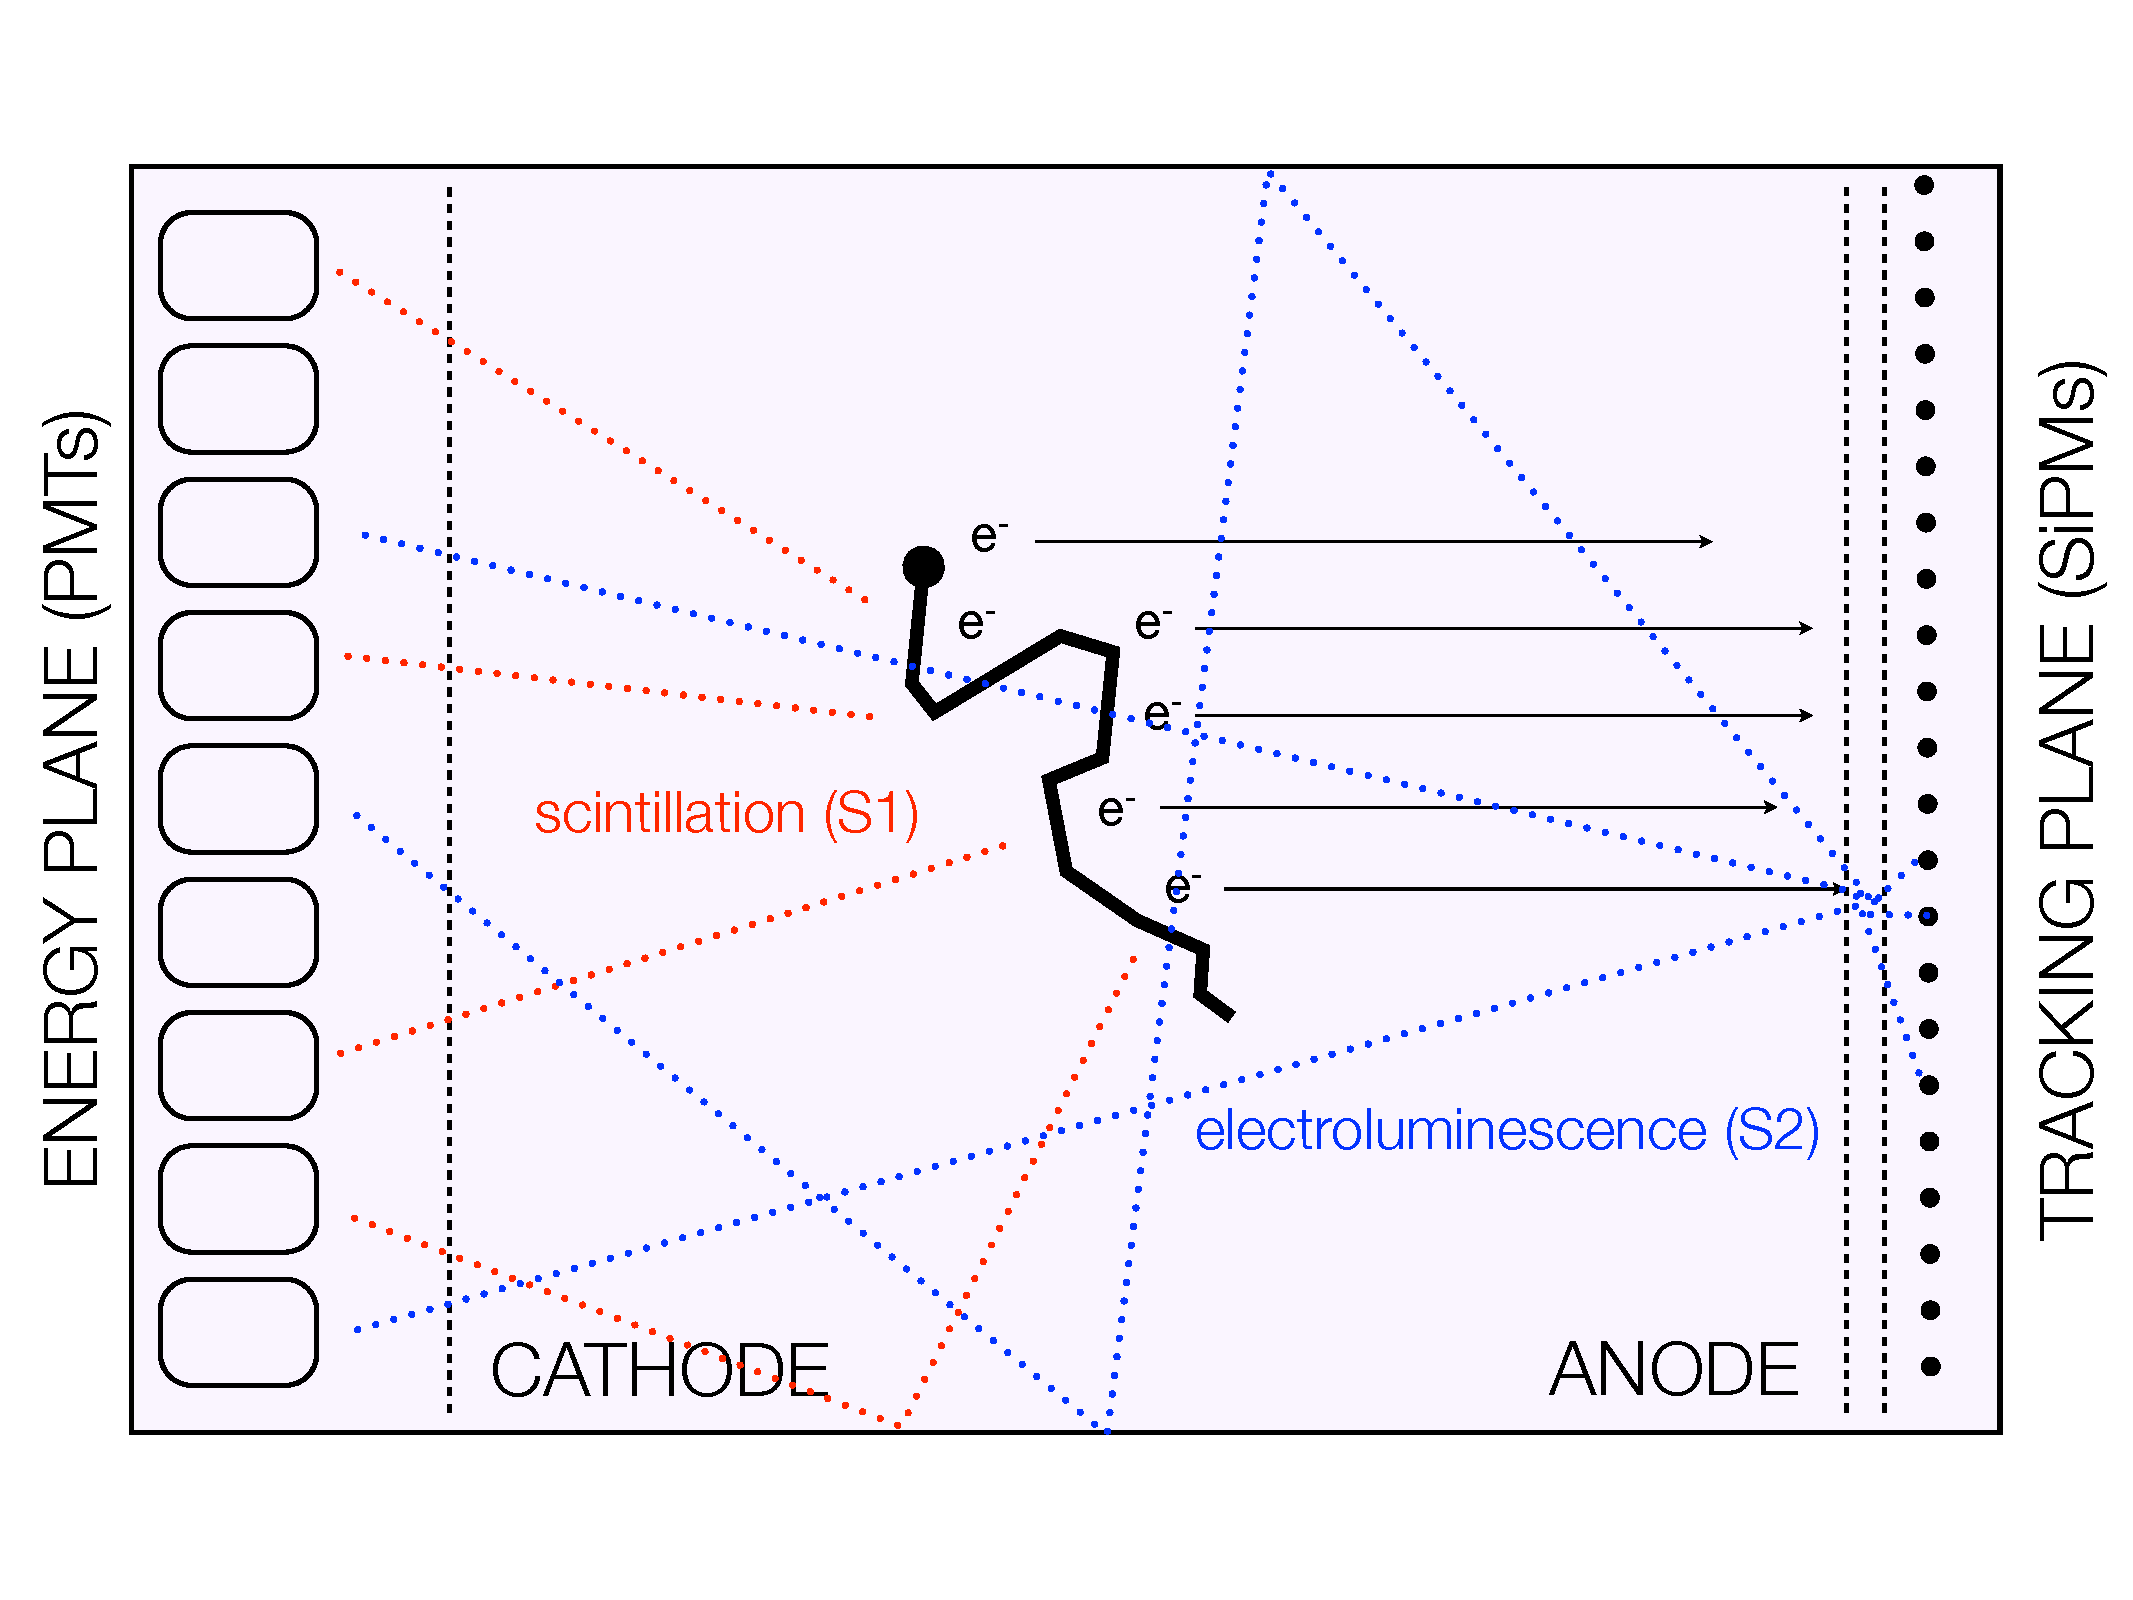
\includegraphics[width= 0.42\textwidth]{fig/nextEL.pdf}
	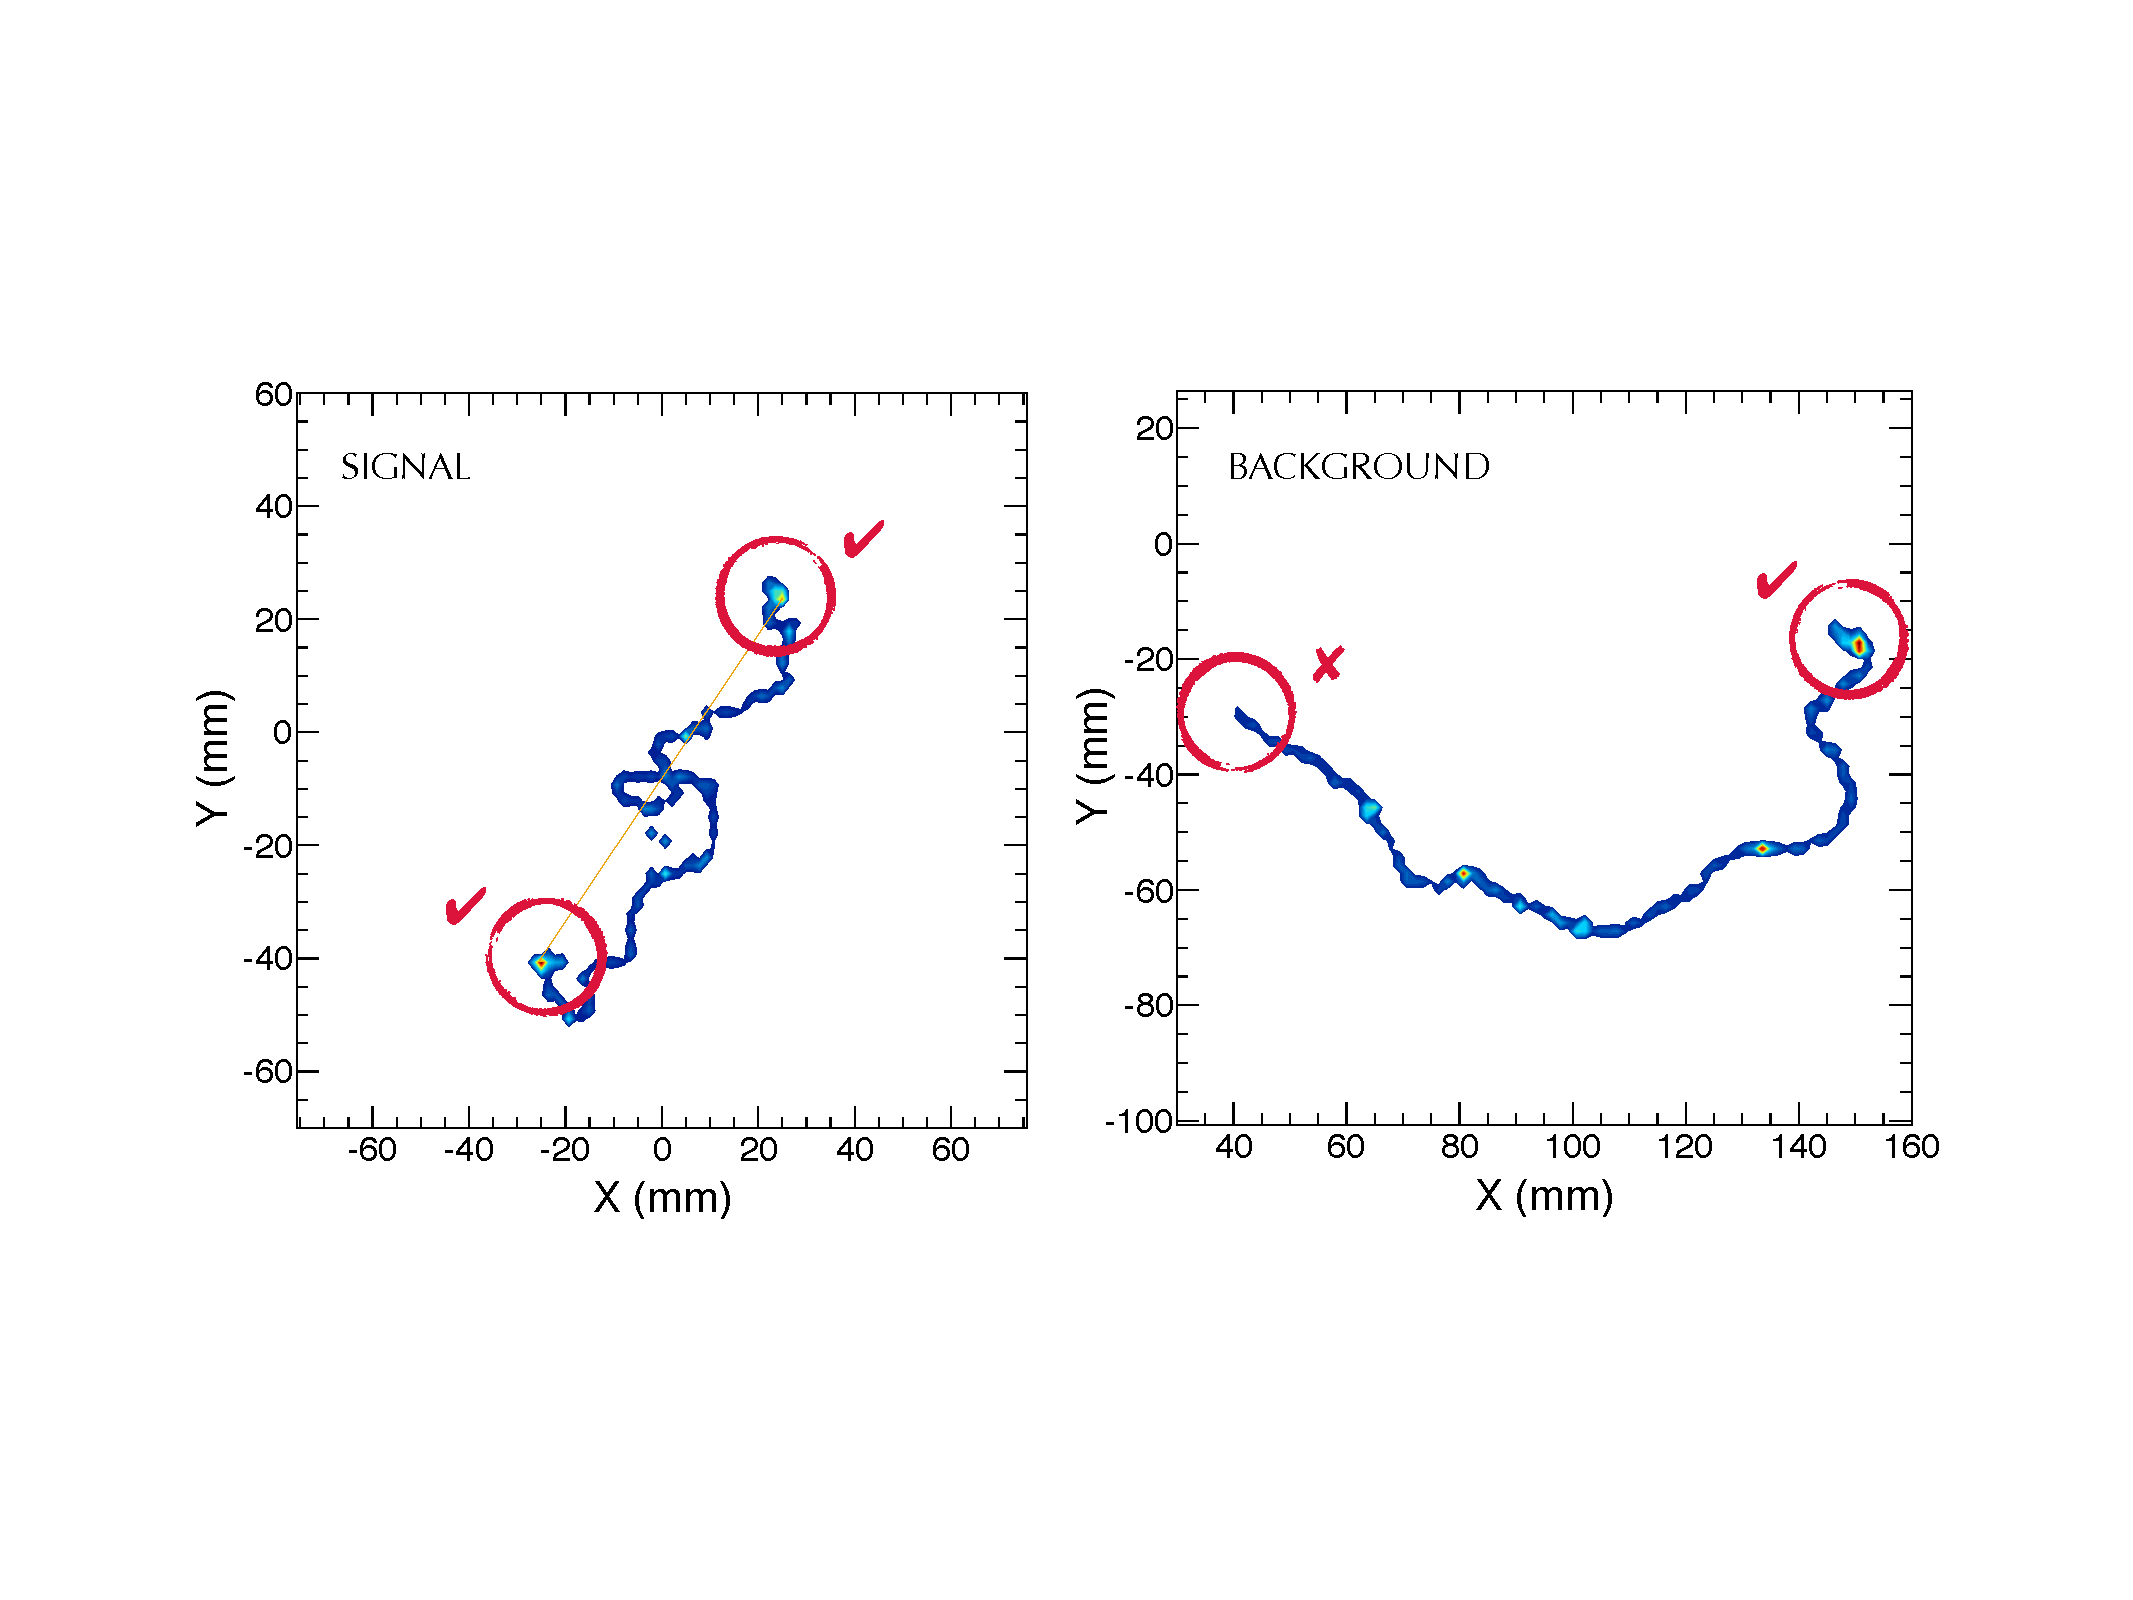
\includegraphics[width= 0.56\textwidth]{fig/TrackSignature.pdf}
	\caption{The NEXT concept. (Left, figure from \cite{Alvarez:2013gxa}) In an asymmetrical EL TPC, energetic electrons produce primary scintillation (S1) and ionization initially, and the ionization is drifted to the EL readout plane and amplified, producing additional scintillation photons (S2).  The energy (PMT) plane detects S1 (coordinate $z$) and S2 (energy), while the finer-resolution tracking (SiPM) plane measures S2 to deduce $(x,y)$ coordinates, resulting in a full 3D reconstruction of the track and its energy. (Right, figure from \cite{NEXT_sensitivity}) The anticipated topologies of signal and background events in a $0\nu\beta\beta$ search with high pressure xenon gas.} \label{fig.SS}
\end{figure}

In order to fully benefit from the potential of the topological signature, a sound procedure for track reconstruction and classification is essential. It has already been shown through a detailed comparison between Monte Carlo and data from the prototype detector NEXT-DEMO that the topological signature can be used to significantly reject background at an allowable cost in efficiency \cite{NEXT_topology}. A Monte Carlo study in \cite{NEXT_DNN} showed that such a topological analysis could be performed significantly better with deep learning techniques.

The conventional NEXT analysis is performed by reconstructing a 3D track in the form of ``hits'' from the pattern of light cast on the tracking plane of SiPM detectors during EL readout. As the EL light arrives at the PMT plane when the ionization electrons of the tracks arrive at the EL plane, the track can be divided into ``slices'' in time and therefore, as drift time is related to axial location within the TPC, in the z-coordinate. The charge detected in each SiPM over each time slice is summed, and from these charges one or more hits are reconstructed by locating the SiPM with the maximum charge, using the charges of neighboring SiPMs in either a weighted sum (barycenter) or 2D Gaussian fit to reconstruct a single point, and repeating this process discarding the charges already considered. The reconstructed volume is then divided into 3D rectangular volumes or ``voxels,'' each of which is filled with the energy of each reconstructed hit that lies within it (see Fig. \ref{fig.recon}). Sequences of connected voxels are denoted as ``tracks'' and multi-track events are discarded.

\begin{figure}[!htb]
	\centering
	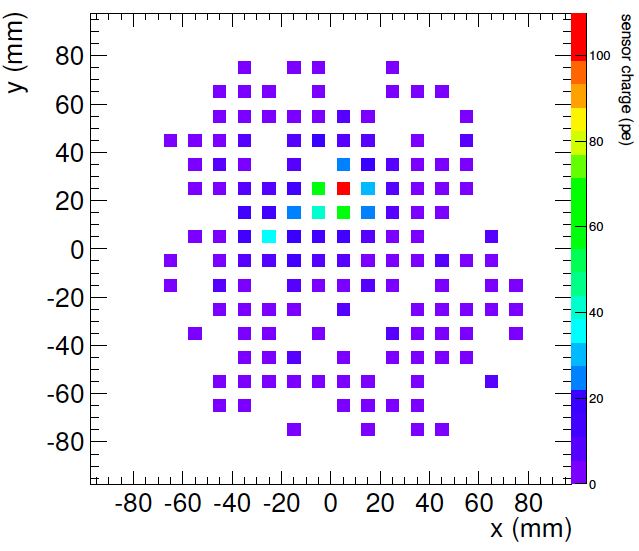
\includegraphics[width= 0.42\textwidth]{fig/sipm_map.png}
	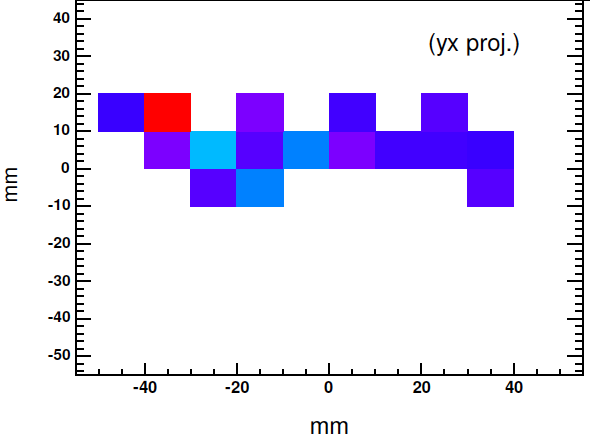
\includegraphics[width= 0.46\textwidth]{fig/xy_proj.png}
	\caption{Conventional NEXT track reconstruction (figures from \cite{NEXT_topology}). (Left) Example of tracking plane signals for a single z-slice in EL readout. (Right) Example x-y projection of a voxelized track produced by a $^{22}$Na gamma source.} \label{fig.recon}
\end{figure}

The analysis continues by considering the single connected track as a graph and using the Breadth First Search (BFS) algorithm to find the shortest path between each pair of voxels in the event. The longest of such shortest ordered paths is considered to be the final track, and the extremes of this path are identified. The energy in the voxels nearby the two extremes can be summed and compared: in cases of signal two larger values (``blobs'') should be found, and only one in the case of background (see Fig. \ref{fig.blobs}).  This algorithm, though reliable in many cases and shown to give good performance, has the major shortcoming that it must operate on a path with a clear beginning and end. Attempts to improve upon this algorithm by applying an external magnetic field and fitting an ordered track to an expected path using a Kalman filter have failed to improve significantly upon the results of the original algorithm despite showing promising results in theory \cite{NEXT_BFIELD}. This is because it was realized that, though in many cases a straightforward ordered reconstruction of an event is obtainable, in a significant number of cases \emph{it is very difficult or impossible to determine the ordering of a reconstructed track.}  This is mainly due to electron multiple scattering, or the sudden changes in course (by large angles) of an ionizing electron due to many scattering interactions with the atoms of the gas.  Such effects produce twisted tracks of varying geometries, often looping back on themselves and crossing. Determining the ordering of an arbitrary event containing multiple crossings is challenging and may require an algorithm that considers many special cases.

\begin{figure}[!htb]
	\centering
	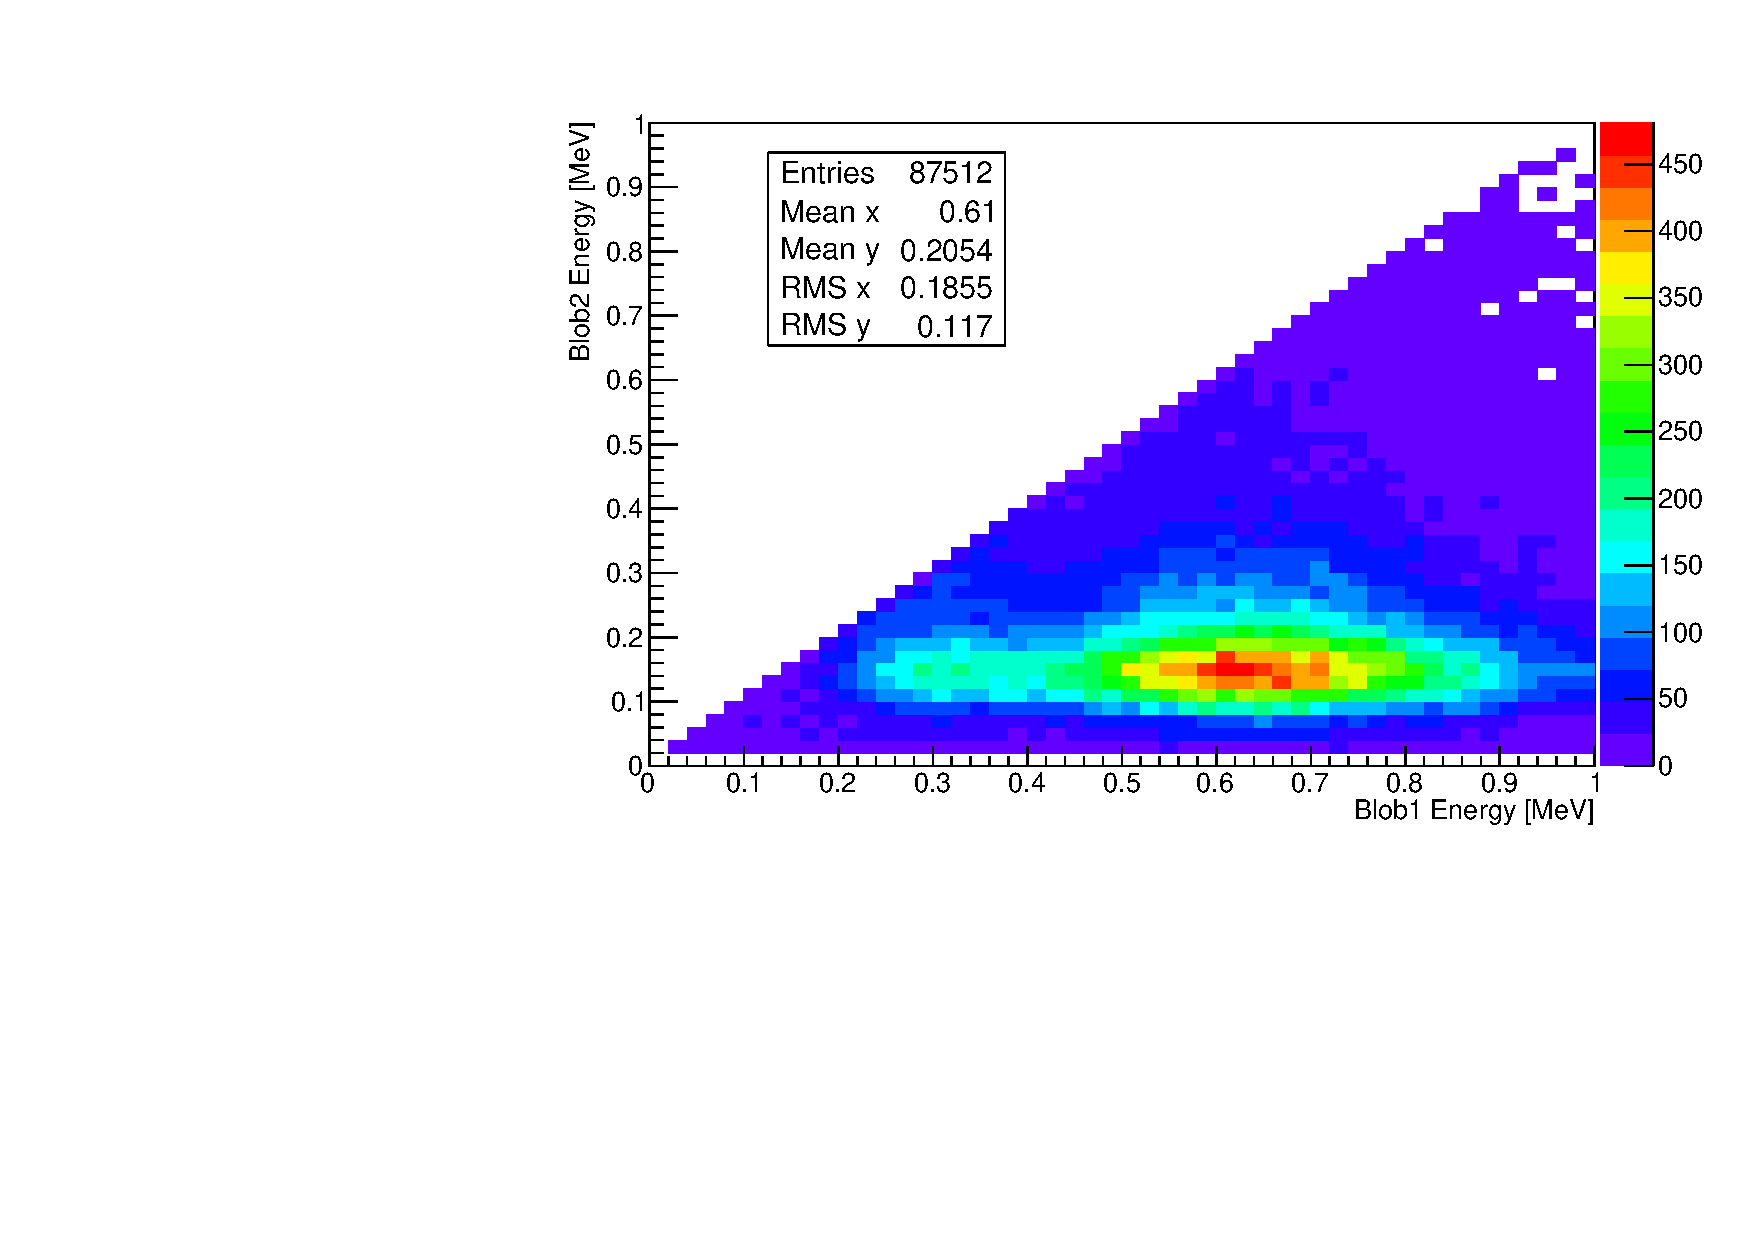
\includegraphics[width= 0.48\textwidth]{fig/blob1vsblob2_Paolina10105_Bi214.pdf}
	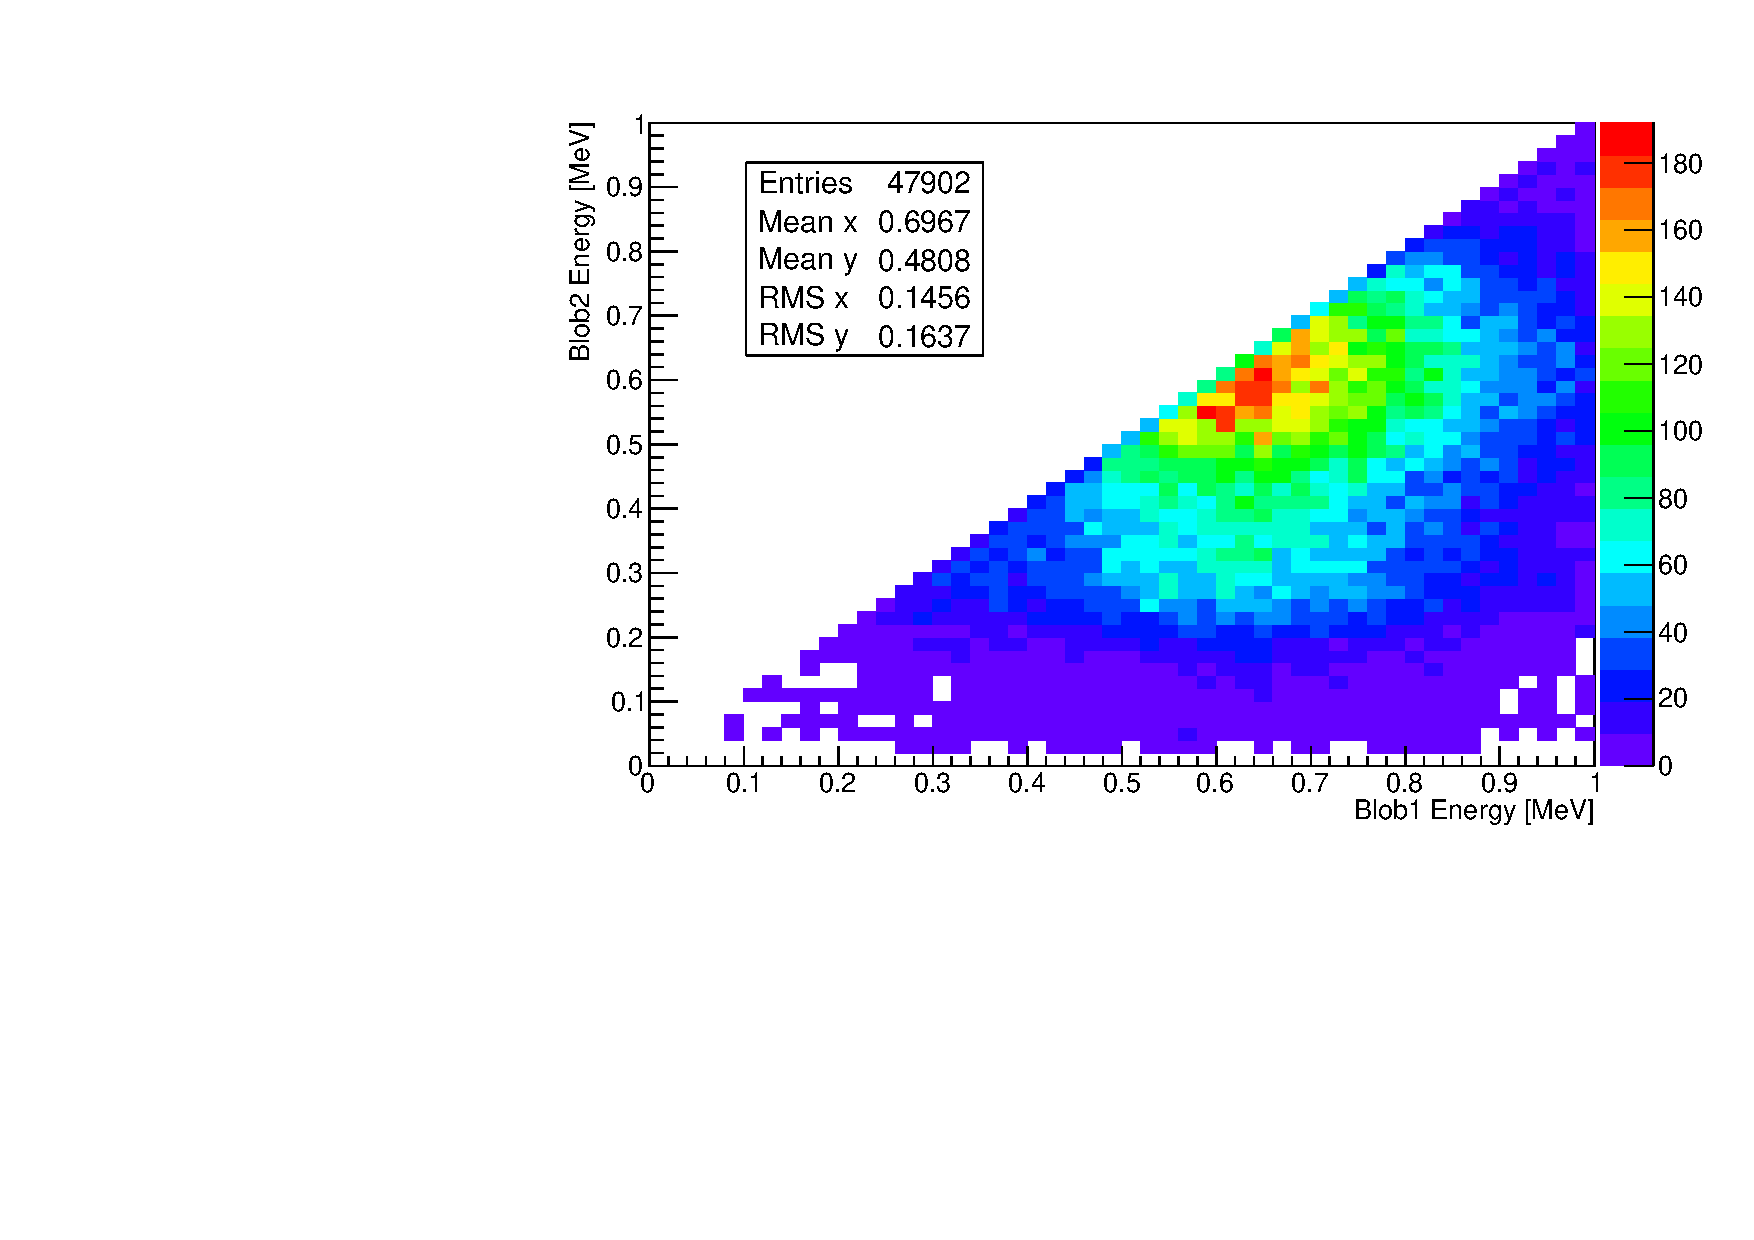
\includegraphics[width= 0.48\textwidth]{fig/blob1vsblob2_Paolina10105_0vbb.pdf}
	\caption{Most energetic blob ($E_{\mathrm{Blob1}}$) plotted against least energetic blob ($E_{\mathrm{Blob2}}$) for simulated background events (left, gamma rays of energy 2.45 MeV emitted in the decay chain of $^{214}$Bi) and signal events (right, $0\nu\beta\beta$ decay). In this example, applying a cut rejecting events with $E_{\mathrm{Blob2}} < E_{\mathrm{cut}}$ rejected all but 11.0\% of background events while keeping 76.6\% of signal events. The full Monte Carlo analysis leading up to these plots is discussed in \cite{NEXT_DNN}. (Figure from \cite{NEXT_DNN})} \label{fig.blobs}
\end{figure}

Performing such an analysis with a DNN does not require pre-determining an ordered path. In some sense the DNN handles this, and as it contains many parameters, it should be able to cover many more special cases than feasible for an analytic algorithm. Replacing the blob-based analysis with a DNN has already been shown to yield significant improvement \cite{NEXT_DNN}. In fact, the DNN does not even require a connected track to operate; the reconstructed z-projections determined in the previous phase of the analysis can be passed directly to the DNN. It is such an analysis that we propose to construct. By presenting a suitable DNN with a statistically broad sample of training events, one should be able to make use of all possible physical information in making the classification decision. We intend to apply such a strategy to obtain the ultimate sensitivity in NEXT and reveal how such an analysis can be applied to similar problems in particle physics.\\

\noindent\textbf{\textbullet\,\,Deep Learning}\\
Neural networks have been used as computational models for over 60 years, but only over the past approx. 10 years have computational advances allowed for creation of neural networks with many layers stacked together, each processing the information output from the previous, known as \emph{deep} neural networks. These networks have given rise to significant advances in complex problems such as recognition of speech \cite{Hinton_2012} and images \cite{Googlenet} due to their ability to extract and process high-level information with their many layers.

The fundamental constituent of a neural network is the \emph{neuron}, which takes some number of inputs $x_i$ and outputs a value $y$ that is some function of its parameters. Its parameters include one \emph{weight} $w_i$ for each input and one \emph{bias} $b$. A value $y = f(\sum_{i}w_{i}x_{i} + b)$ is computed by the neuron, where $f$ is called the activation function and is normally chosen to be a nonlinear function such as the sigmoid function $\sigma(z) = (1 + e^{-z})^{-1}$. In a conventional neural network consisting of fully connected layers, the outputs of each neuron in one layer are input to each neuron in the next layer. To train the network, a training sample consisting of inputs and the expected outputs is produced, and the net ``learns'' by introducing the inputs to the input layer, propagating all values through the neurons of the net, and computing a \emph{loss function} which quantifies the error between the actual and expected values in the output layer. The weights and biases in all of the neurons in the network can then be adjusted in a manner that serves to minimize the loss function, bringing the net closer to convergence. This is commonly done by first adjusting the parameters of the output layer and passing the information about how the loss function changes with respect to the outputs of each layer backwards through the network, i.e. via \emph{back propagation}. One common optimization method which seeks to tune the net in the direction of decreasing loss is \emph{stochastic gradient descent}. In this method and variations, the derivative of the loss function is estimated based on small random samples or \emph{batches} of training data. Training a network is then an iterative process which occurs in small batches, each of which seeks to drive the network to a state in which the loss function is overall lower. Events from the training sample are selected randomly to construct the batches, and are only used once until all training samples have been presented to the net, or an \emph{epoch} of training has been completed, at which point the process continues with another epoch.

\begin{figure}[!htb]
	\centering
	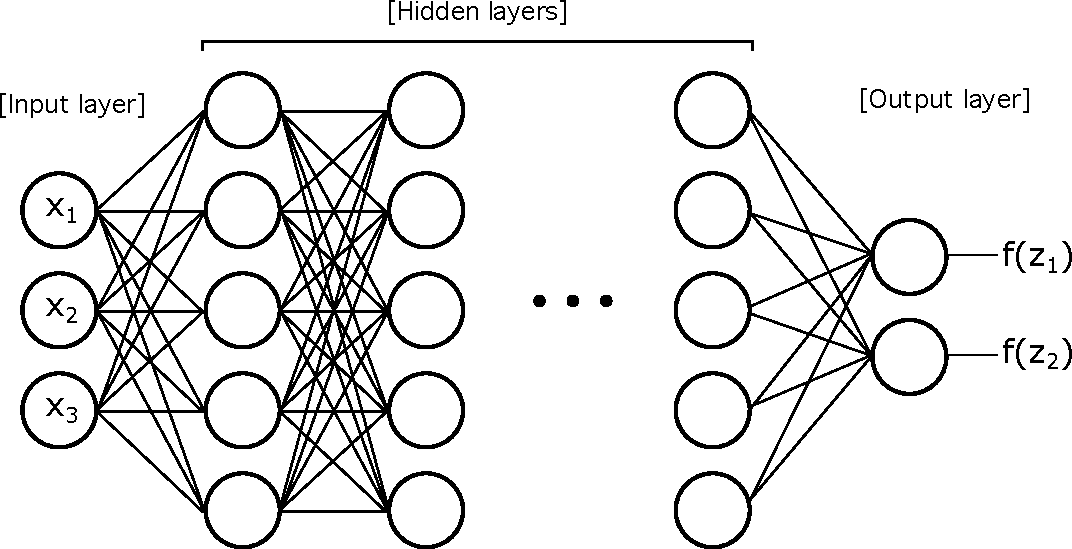
\includegraphics[width= 0.48\textwidth]{fig/general_nn_fc.pdf}
	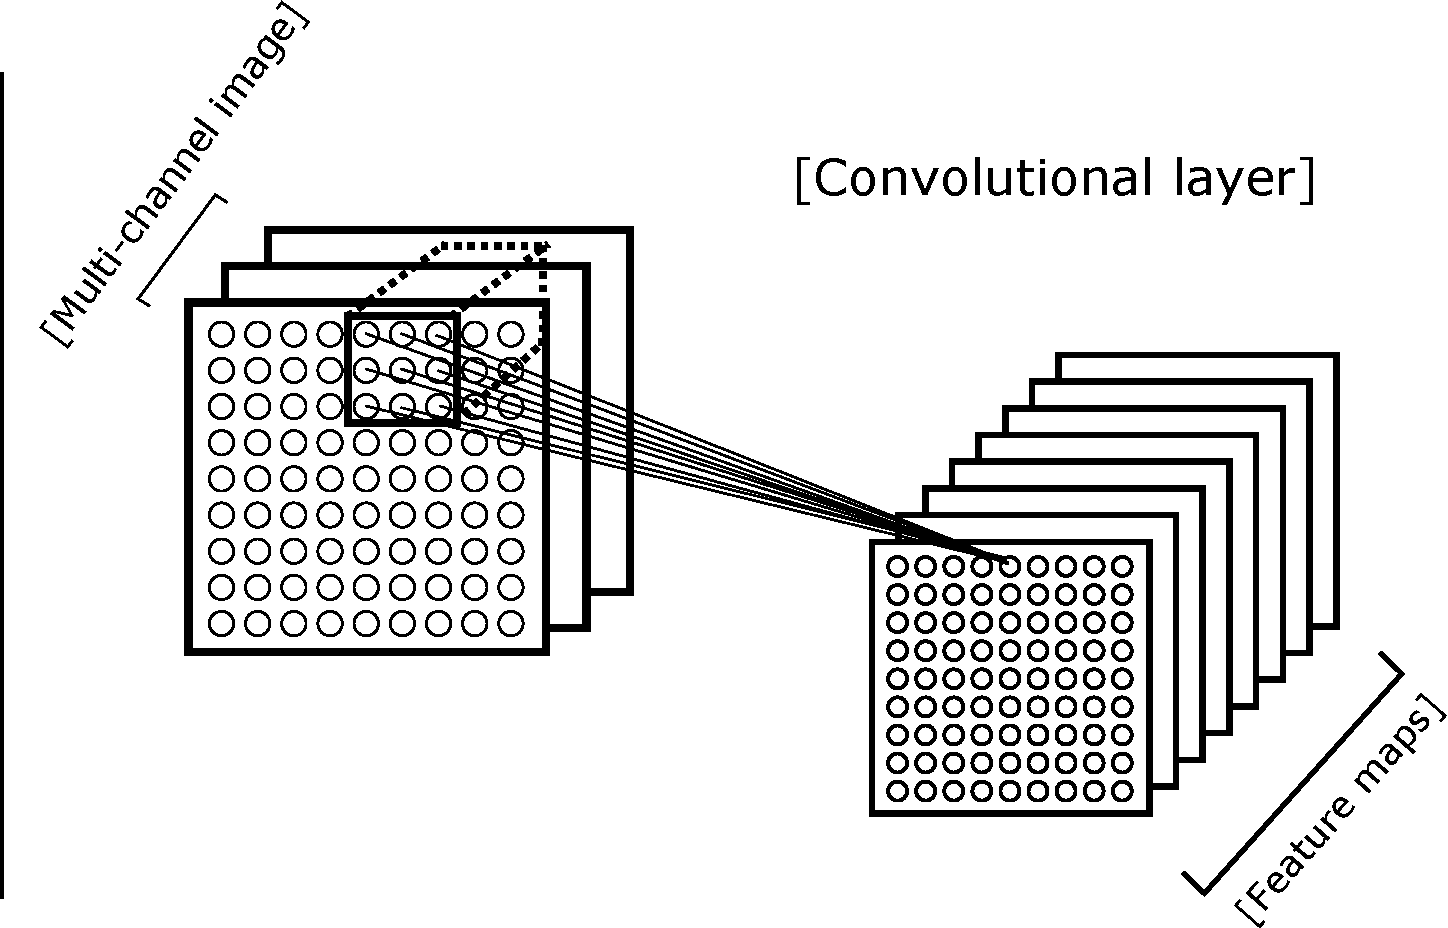
\includegraphics[width= 0.48\textwidth]{fig/cnn_example.pdf}
	\caption{(Left) A fully-connected neural network architecture in which all neurons in a layer are connected to all neurons in the previous and next layers. (Right) A convolutional layer, in which the neurons consider as inputs only those within an $m \times n ~(\times ~k_i)$ for a filter size of $m \times n$ and a number of input channels $k_i$. The number of output channels $k_f$ is the number of ``feature maps,'' roughly corresponding to the number of ``features'' the layer is trained to identify. Each neuron in each output channel shares the same set of $m \times n ~(\times ~k_i)$ weights, significantly reducing the number of parameters when compared to a fully connected layer. (Some content of figure from \cite{NEXT_DNN})} \label{fig.nets}
\end{figure}

In the era of deep learning, conventional neural networks have evolved to suit individual problems and take advantage of the ability of modern computers to train a many-layer network. A \emph{convolutional neural network} (CNN) is one in which one or more specialized convolutional layers are present. These layers are not fully connected, but only a subset of outputs from the previous layer are used as inputs to each neuron in a convolutional layer. The outputs are then constructed with a set of weights and biases that are shared across all neurons in the layer. For example, in a 2D convolutional layer, the inputs are transformed to an image of dimensions $l \times w$. Some number $k$ of \emph{filters}, or sets of weights and biases of dimension $m \times n$ are applied to each patch of $m \times n$ input neurons via a multiplicative sum (convolution). An activation function is applied to the result of each convolution to give an output value so that for each filter $k$, a \emph{feature map} is generated which describes the response of the input images to the filter. As the net is trained, the filters begin to identify certain features of the image by outputting higher output in their feature maps as they are encountered. Deeper convolutional layers can become capable of identifying yet higher-level features. Several techniques are used in conjunction with convolutional layers, including \emph{pooling} which reduces the size of a feature map by taking some value (the average or the maximum) of subsets of the neurons in the feature map and discarding the rest, thus reducing the number of parameters in deeper layers. 

An initial study \cite{NEXT_DNN} has shown that CNNs provide an improved alternative to the NEXT conventional (``blob''-based) analysis. The GoogLeNet \cite{Googlenet}, a 22-layer deep CNN recently developed to identify objects in images, was trained on over 400 000 Monte Carlo events (50\% single-electron background, 50\% $0\nu\beta\beta$ signal) using the Caffe deep learning framework \cite{jia2014caffe} and the NVIDIA DIGITS \cite{DIGITS} interface. The trained nets were then used to classify the same events as those to which the conventional analysis was applied (figure \ref{fig.blobs}) and was found to perform better by a factor of 1.17 - 1.62 depending on the reconstruction resolution (size of voxels). This analysis was performed by creating a color image from three projections (xy, xz, yz) of the voxelized track and using the resulting 2D image as input to the GoogLeNet. As standard out-of-the-box tools were used in this initial analysis, there is potential for significant improvement with further study. In particular, optimizing and understanding the design of the classifier neural network, replacing the standard NEXT reconstruction methodology (voxelization + graph theory) with a DNN, and creating a complete DNN-based analysis chain all promise potential improvement and lie within the objectives of this proposal.

There is also strong potential for revealing additional applications of deep learning in particle physics. Several other studies have already made use of deep learning and obtained positive results. In \cite{Aurisano_2016}, a CNN was designed to classify reconstructed neutrino events in the NOvA experiment into one of several categories based on the flavor of the interacting neutrino and the type of interaction that occurred, and the results were found to be on-par and in some cases better than those of the previously employed algorithms. In \cite{Baldi_2014}, 5-layer deep neural networks were shown to perform significantly better than single-hidden-layer neural networks in classifying signal vs. background in a Monte Carlo study of two benchmark high-energy physics classification problems. They even concluded that the deep neural networks showed signs of learning higher-level features from the simulated data.\\

{\noindent\textbf{Section B: Methodology}}\\
The proposed actions to be carried out can be divided into three main phases which consist of: 1. optimization of the DNN-based analyses for event classification and reconstruction, 2. the demonstration of the full background rejection potential in NEXT-NEW, and 3. construction of a full DNN-based analysis chain for use on data from NEXT-100. By the end of the proposed project, we intend to have demonstrated how DNNs can be used to perform substantial physics analyses, replacing and improving upon conventional analysis algorithms, and have applied the DNN-based analysis to data from NEXT-NEW and NEXT-100. This should lead to a solid understanding of how to confront a tonne-scale search for $0\nu\beta\beta$ decay.\\

\noindent\textbf{\textbullet\,\,Phase I - Optimization of DNN-based analysis (1 - 1.5 years)}\\
The two major aspects of the NEXT analysis that could be significantly improved with the use of DNNs are the \emph{classification} and \emph{reconstruction}. While some initial results have been obtained demonstrating improved classification, further studies are still required to fully understand the potential for improvement. Only very basic attempts at a DNN-based reconstruction have been made at this point, and, due to uncertainties introduced by diffusion in pure xenon gas, reconstruction resolutions of no better than approx. 1 cm in $(x,y)$, 0.5 cm in $z$ are currently realizable experimentally. However, studying more optimistic resolutions cases under the assumption that a low-diffusion gas (pure xenon + a coolant gas) is employed will be important for phase II where resolutions as low as 0.2 cm in $(x,y,z)$ may be realizable. Though the studies to be undertaken in this initial phase of the project will be the focus for the first 12 - 18 months, it will be relevant for the entire time, as the studies addressed may be revisited in later phases.

To perform DNN-based classification from a reconstructed track, the information of the reconstruction must be passed to the net as input, and the net's decision must be communicated as output. In previous studies, the 3D region of space containing the track has been voxelized such that the reconstruction is a set of voxels, each containing some amount of energy. This information was then projected onto the $xy$, $yz$, and $xz$ planes (see figure \ref{fig.projs10105}), and the energies in each projected (now 2D) voxel were treated as the color channel, $(xy, yz, yz) \rightarrow (R, G, B)$ of a color image. These images could then be used with the GoogLeNet using software tools already developed to perform image recognition. The inputs to the net were the individual pixels of the 2D image, and the output layer was 2 neurons which were given a \emph{softmax} activation function - one in which the weighted sum of inputs of each of the two neurons is exponentiated, and the sum of the two exponentiated values is normalized. 

\begin{figure}[!htb]
	\centering
	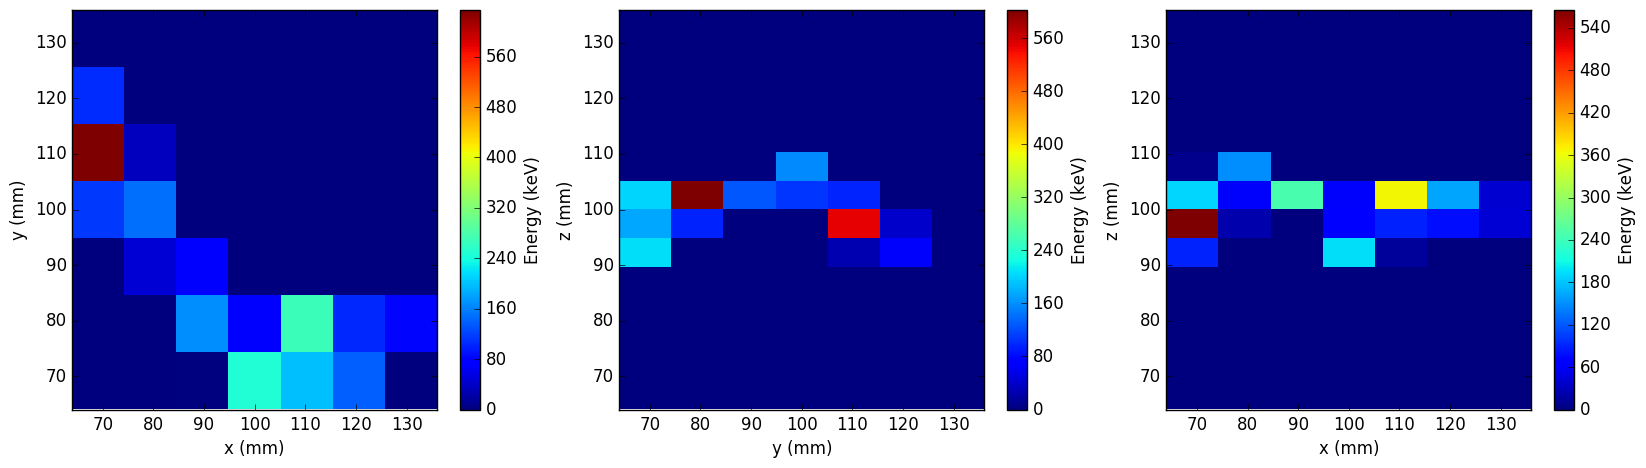
\includegraphics[scale=0.4]{fig/plt_h2D_dnn_NEXT100_0vbb_si_v10x10x5_r200x200x200_6_si.png}
	\caption{\label{fig.projs10105}Projections in xy, yz, and xz for an example signal event voxelized with $10 \times 10 \times 5$ mm$^3$ voxels.}
\end{figure}

In further studies, several changes to this strategy could be investigated. For example:

\begin{enumerate}[itemsep=-1mm]
	\item[-] First, the structure of the neural net could be modified from that of the GoogLeNet to that of a less complex CNN and tuned more towards the problem at hand. The GoogLeNet was designed to identify complex features in everyday images, but for identifying patterns in voxelized tracks, perhaps the ``22-layer deep'' architecture is unnecessary and a shallower net with more convolutional filters at earlier stages should be developed. 
	\item[-] It may be useful to analyze the three projections in separate parallel subnets, similar to the strategy used in \cite{Aurisano_2016} rather than treating them initially as three channels, which implies that their information is combined early on after an initial convolution. 
	\item[-] 3D convolutional layers could be employed, which, though more computationally expensive, do not suffer from the loss of information present when taking projections.
\end{enumerate}

To implement the ideas above, the DNN software Keras \cite{Keras} in combination with Theano \cite{Theano} and Tensorflow \cite{Tensorflow} can be used to rapidly create and train prototype DNNs. It will also be of great interest to attempt to understand what the net is ``learning'' to optimize the net design. This can be done by examining the values of the weights of key convolutional layers, which give insight into what features they are extracting, and by carefully examining the events that are improperly classified in an attempt to identify features that are not being considered by the net. There are also physical limits to the problem - for example, a $0\nu\beta\beta$ event in which nearly all the energy is carried away by one of the two electrons is, to a detector of finite resolution, physically equivalent to a single-electron (background) event. Understanding such details not only helps in converging on the best possible classification in NEXT but also will guide similar applications of DNNs in physics.

The reconstruction of tracks using DNNs could serve as a replacement for an otherwise complex reconstruction algorithm that would need to consider many special cases. As mentioned previously, due to electron multiple scattering, electron tracks in xenon gas can become quite complex. As the events are reconstructed as a series of 2D projections, a single projection may contain one or several regions of energy deposition. Assigning a single ``point'' of energy deposition to each of such regions may give a good representation of the track, but in many cases such regions will be more suited to a line than a point, and a more sophisticated analysis is needed. A good algorithm must decide where the energy was deposited and how much was deposited there by looking at a map of SiPMs, which in NEXT-NEW will be positioned with a pitch of 1 cm (see figure \ref{fig.reconst_example}).

In NEXT, the individual electrons of an ionization track will arrive at the EL plane at some time $t$ and location $(x,y)$ and produce some amount of EL light detected by the SiPMs of the tracking plane and the PMTs of the energy plane. Therefore, one can imagine, summing the energy of all ionization electrons arriving within a time range $t \in [t_1,t_2]$, one has an energy distribution in the $xy$ plane. Such a distribution will cast a specific pattern of light on the tracking plane, and the ideal reconstruction algorithm would deduce this distribution exactly from the measured SiPM responses. While the conventional NEXT algorithm may need to make several decisions including how many points to reconstruct for a given SiPM response map and how to use the information from the SiPMs to determine where to locate that point, a DNN-based approach is straightforward: the response of each SiPM constitutes one input neuron, and each pixel on the energy distribution grid is an output neuron. The output layer has softmax activation as in the classification problem, so the sum of the values in all output pixels is 1 and can be multiplied by the total energy of the slice (determined by the energy plane). A track is then a series of reconstructed slices. The net can be trained on many slices taken from Monte Carlo generated tracks, in which the true 2D energy distribution of the slice is known (see figure \ref{fig.reconst_example}).

\begin{figure}[!htb]
	\centering
	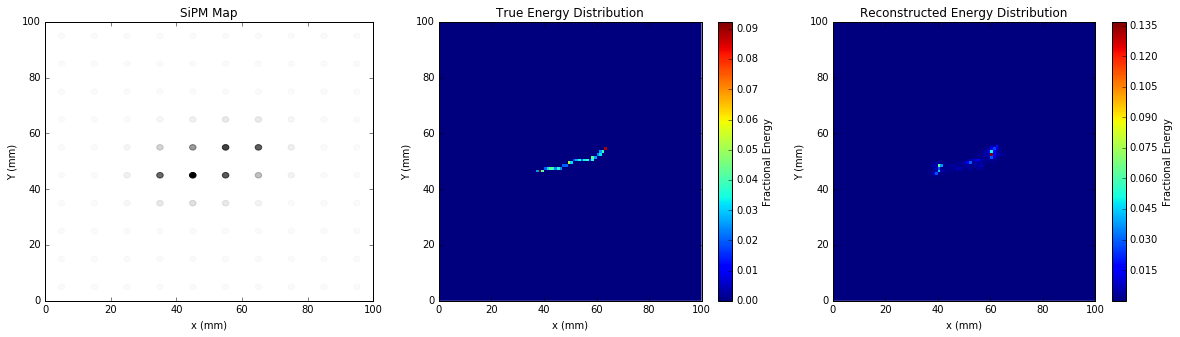
\includegraphics[scale=0.41]{fig/reconst_example_evt1.png}
	\caption{\label{fig.reconst_example}Example of reconstruction of a single slice. The normalized SiPM map (left) produced by the true energy distribution (middle), as reconstructed by a simple CNN (right).}
\end{figure}

A detailed study of DNN-based reconstruction would be conducted using this strategy. Several challenges still remain, such as determining the optimum DNN architecture for the problem and dealing with the very large number of output neurons that would be required to cover the entire tracking plane with fine resolution.

Though visual reconstruction of particle tracks is a primary goal of NEXT and will be a principle part of the analysis, it may not be necessary for a DNN-based classification. If a DNN is to be used to reconstruct the energy distribution produced by a track in a 3D voxelized space, and the resulting voxels are to be input to another DNN to perform the classification, perhaps a single net could be given as input the SiPM maps corresponding to the z-slices and output the classification. Such an analysis must also be studied, as it is less intuitive. If sucessful, it would further demonstrate the power of DNNs to replace conventional analysis algorithms - we reconstruct the tracks and make the classification decision based on the track because this is the most sensible manner in which we can break down and approach the classification problem. For a DNN, as long as the same original information (the SiPM response maps) is present, it can ``learn'' its own way to use that information to make the optimal classification. As the reconstruction step introduces some error, this may be the ideal approach.\\

\noindent\textbf{\textbullet\,\,Phase II - Demonstration of full background rejection potential with NEXT-NEW (2 years)}\\
One important upgrade to the NEXT technology that will be addressed in the coming years is the use of a low-diffusion gas mixture. An important factor limiting the ultimate reconstruction resolution is the diffusion experienced by the ionized electrons as they drift towards the EL plane. Because of this, events produced far from the EL plane do not strike the plane at the exactly the $(x,y)$ location at which they were produced, nor do they arrive at a time corresponding to the exact $z$-location at which they were produced, but these coordinates are smeared by diffusion in a Gaussian manner with $\sigma \sim 10 ~\mathrm{mm} / \sqrt{\mathrm{m}}$. The reconstruction resolution is extremely important in obtaining optimal background rejection with DNNs, as was found in an initial study (see figure \ref{fig.svsbDNN}).

\begin{figure}[!htb]
	\centering
	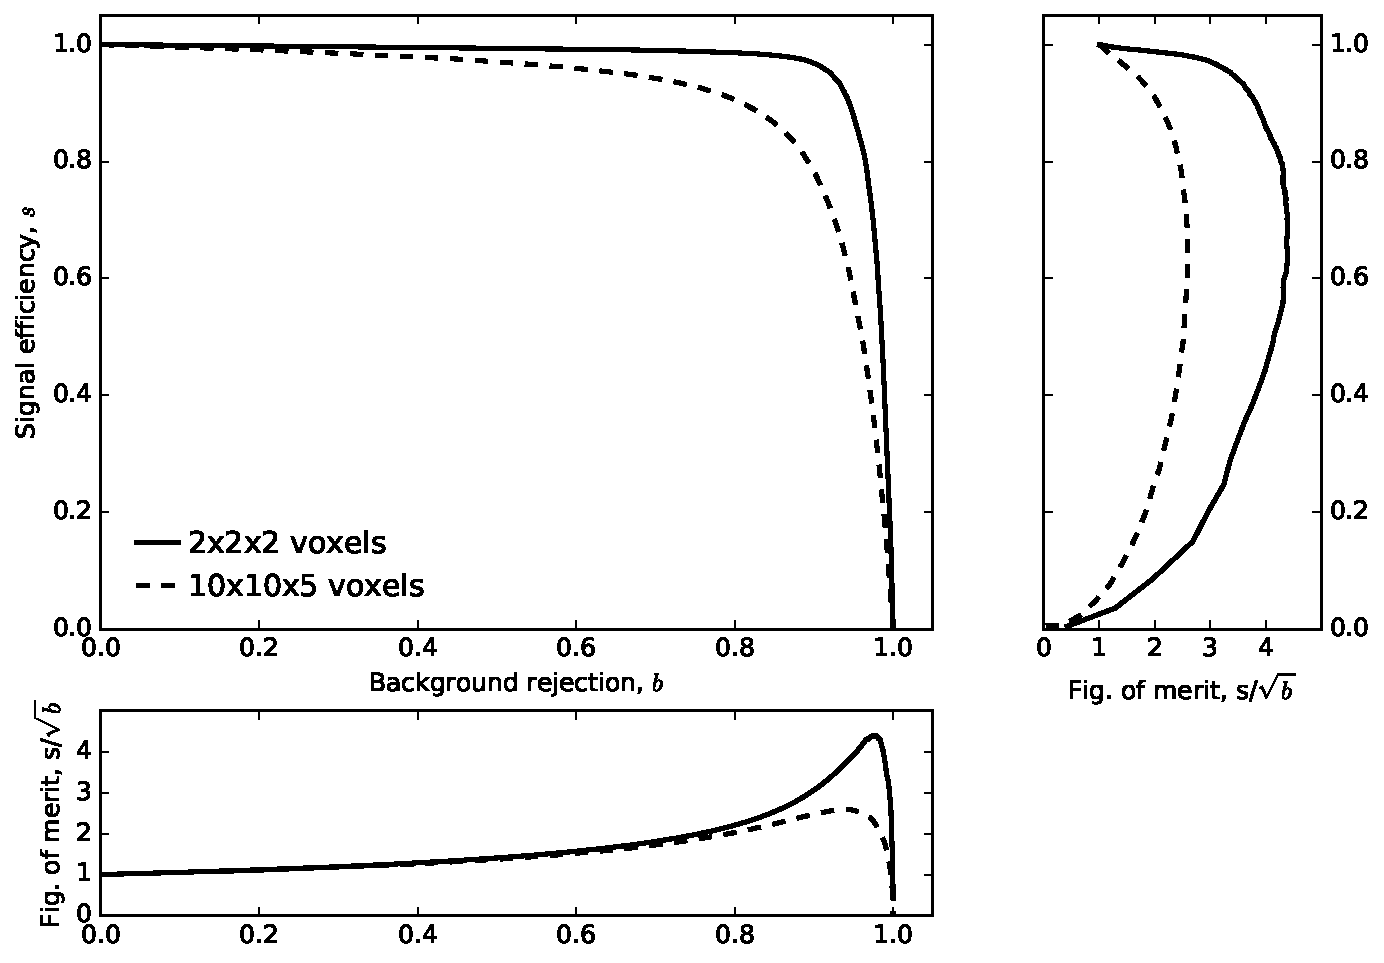
\includegraphics[scale=0.5]{fig/sigvsbg_DNN.pdf}
	\caption{\label{fig.svsbDNN}Signal efficiency vs. background rejection for a DNN-based classification of Monte Carlo events with different reconstruction resolutions, along with a figure of merit which follows the sensitivity to $0\nu\beta\beta$ decay. The energy in each event was distributed into 3D volume elements (voxels) with sizes that reflect roughly the reconstruction resolution. Better resolution offers significantly more potential for background rejection and an ultimately higher sensitivity. (Figure from \cite{NEXT_DNN})}
\end{figure}

Recent Monte Carlo simulations within the NEXT collaboration (ref?), have shown that adding small amounts of a ``coolant'' gas to the pure xenon could significantly reduce the diffusion without significantly affecting the electroluminescent properties of the gas. After its initial physics operation (expected to end in 2018-2019?), NEXT-NEW will be available for a low-diffusion study to which a candidate gas additive, such as CH$_4$ or CF$_4$, could be added, and techniques developed in phase I could be applied to compare reconstruction and classification in the standard-diffusion and low-diffusion cases. Such a study would seek to demonstrate a factor of order 10 improvement in background rejection from a combination of an improved analysis and low diffusion, and would involve:

\begin{enumerate}
	\item[1.] Operation of NEXT-NEW with the low-diffusion gas mixture. This may involve minor changes in detector hardware configuration, particularly in the gas recirculation system, but should otherwise be straightforward. The collaboration will have gained the necessary experience to make this transition smoothly.
	\item[2.] Calibration of the detector under conditions of low diffusion. The resolution of the detector in reconstruction of a single point can be measured using point-like energy depositions produced by x-rays of energies 9 keV and 30 keV produced by a $^{82}$Kr radioactive source. These points can be reconstructed using a DNN trained on Monte Carlo events as shown in figure \ref{fig.reconst_example}, and/or by a similar DNN which reconstructs a single point rather than an image. In addition to quantifying the single-point resolution of the detector, this data is also used in conjunction with the information measured at the energy plane to produce a table of coefficients to provide corrections to the energy due to the effects of the detector geometry on the amount of light collected. The improved position resolution as well as improvements in reconstruction with the use of DNNs therefore lead to better energy corrections and thus improved energy resolution.
	\item[3.] Demonstration of the reconstruction and background rejection capabilities of the DNN-based analysis using calibration sources. The procedure would be similar to that employed in \cite{NEXT_topology}, in which ``background'' events are produced by 1.275 MeV gamma rays from a $^{22}$Na source, and ``signal'' events are electron-positron pairs of total energy 1.592 MeV produced via pair-productions in the interactions of a 2.614 MeV gamma ray from a $^{228}$Th source (in which both 511 keV gammas produced in the annihilation of the positron escape from the active volume).
\end{enumerate}

We aim to demonstrate a factor of 10 background rejection from the current conventional analysis for an acceptable signal efficiency using a DNN-based analysis under conditions of low-diffusion. Though this is an aggressive goal, \emph{we have already shown in an initial study that in the low-diffusion case, we expect to achieve a factor of 1.6 improvement solely by replacing the conventional ``blob'' cuts by a DNN classifier.}\\

\noindent\textbf{\textbullet\,\,Phase III - Construction of a full DNN-based analysis for NEXT-100 (1.5 - 2 years)}\\
The final phase of the proposed project consists of applying what was learned in the first phases to the development of the analysis for NEXT-100. Such an analysis would employ DNNs at several stages. In each case, the net would be trained with many suitable Monte Carlo events. As NEXT-100 will contain significantly more sensors than NEXT-NEW (60 as opposed to 12 PMTs, and of order 7200 as opposed to 1800 SiPMs) and therefore produce larger volumes of data, more powerful computer hardware, described in section C, will be employed in the analysis. The analysis can be divided into several key steps, including pre-processing, reconstruction, and classification. Calibration steps outside the main analysis chain will also be necessary. These steps are summarized below and sketched in figure .\\

\noindent\textbf{Pre-processing:} Here the raw data from the detector is processed from waveforms, or voltage samples vs. time from the PMTs and SiPMs, to sensor response maps, or charge in detected photons for each sensor in slices of time. This step involves integration of the signals in each sensor and conversion to photons using light calibration information. An initial energy cut can be applied at this point to eliminate events that fall well outside the energy range of interest.\\

\noindent\textbf{Reconstruction:} The spatial distribution of energy in the event (the particle track) is determined from the patterns present in the SiPM sensor maps and the energy information from the corresponding PMT sensor maps using a DNN. Conversion factors and geometrical corrections determined from the energy calibration step are then applied to give a fully reconstructed track with position and energy information.\\

\noindent\textbf{Classification:} A DNN is used to classify the event as signal or background. Depending on the results of the studies in the previous phases, the DNN may make use of the position information obtained from the reconstruction step or use the corrected SiPM sensor maps directly.\\

\noindent\textbf{[Calibration:]} Separate calibration steps will need to be run, including a light calibration in which LEDs are used to determine the single-photon response of each sensor, and an energy calibration step using point-like depositions to determine the conversion between photons detected in the energy plane and physical energy, and to determine geometrical corrections. Higher-energy sources may also be used in the energy calibration step to confirm linearity. A DNN will be used to reconstruct point-like energy depositions and thereby extract the geometrical correction factors.\\

\begin{figure}[!htb]
	\centering
	
\includegraphics[scale=0.18]{fig/analysis_diagram.pdf}
	\caption{\label{fig.analysis}Summary of DNN-based analysis chain for application to NEXT-100. The steps requiring DNNs specifically are shaded in gray.}
\end{figure}

Our ultimate goal in this phase is to demonstrate the potential improvement in sensitivity to $0\nu\beta\beta$ decay from the combination of using DNNs and possibly reduced diffusion. Figure shows the potential improvement obtained from low diffusion and the use of DNNs for classification in the recent Monte Carlo study \cite{NEXT_DNN} performed by NEXT. All in all, we emphasize that in order to surpass values of $T^{0\nu}_{1/2}$ near $10^{27}$ years, it will require a combination of improved analysis and possibly lower diffusion, and an active mass of order tonnes.\\

\begin{figure}[!htb]
	\centering
	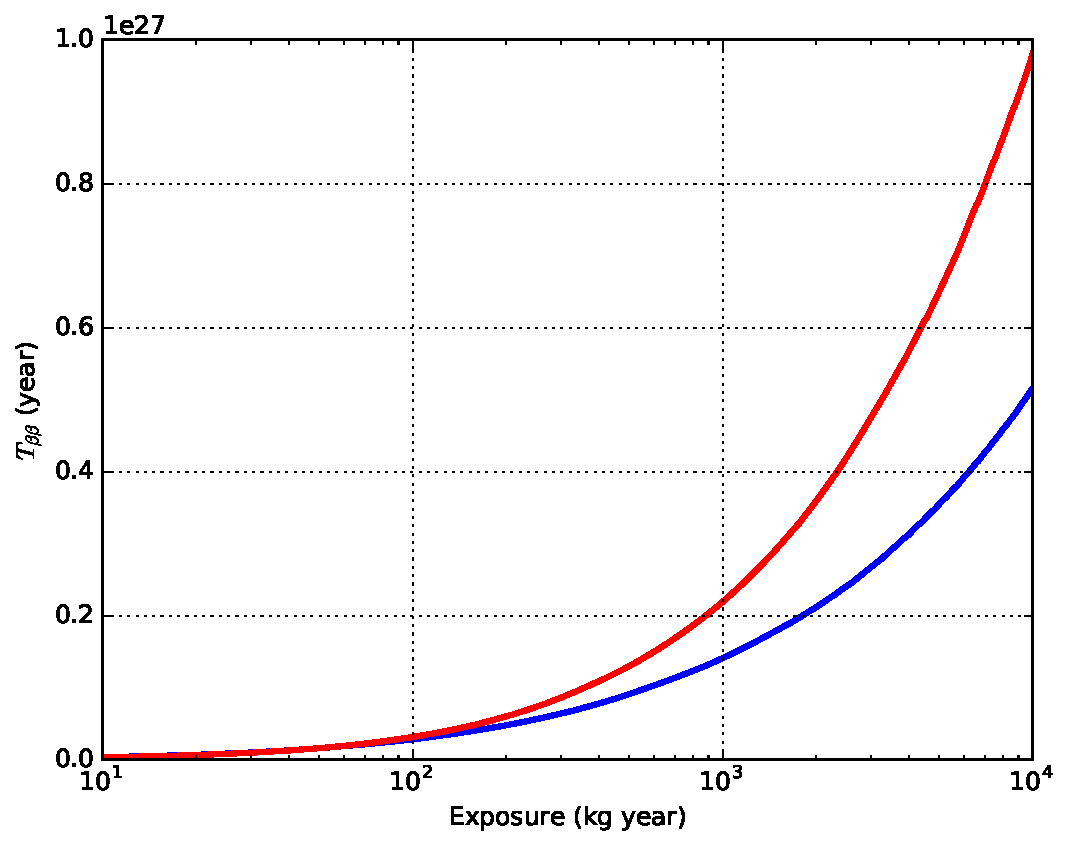
\includegraphics[scale=0.5]{fig/half_life_sensitivity.pdf}
	\caption{\label{fig.halflife}The calculated sensitivity of NEXT-100 to the half life of neutrinoless double beta decay $T^{0\nu}_{1/2}$ for a given exposure time. The blue curve shows the sensitivity assuming the conventional NEXT analysis under conditions of pure xenon diffusion, and the red curve shows the sensitivity assuming the improvements obtained thus far with DNN-based classification and low diffusion. The calculation was done using the Feldman-Cousins approach \cite{Feldman_1998} as described in detail in \cite{NEXT_sensitivity}. (Figure from \cite{NEXT_DNN})}
\end{figure}

{\noindent\textbf{Section C: Resources (including project costs)}}\\

\noindent\textbf{\textbullet\,\,The NEXT Collaboration}\\
NEXT is an international collaboration consisting of groups from over 15 institutions and 5 different countries. It is lead by co-spokespersons J.J. G\'{o}mez-Cadenas (Research Professor, Consejo Superior de Investigaciones Cient\'{i}ficas (CSIC), Spain) and David Nygren (Presidential Distinguished Professor of Physics, University of Texas at Arlington (UTA), USA). G\'{o}mez-Cadenas founded the neutrino group at the Instituto de F\'{i}sica Corpuscular (IFIC) in 1998, which now consists of 2 full professors, 2 staff scientists, 4 postdocs, 6 graduate students, 2 electrical engineers, and 2 mechanical engineers. Nygren is the inventor of the Time Projection Chamber (TPC), a detector technology which has made tremendous impact on the field of particle physics, and is a member of the National Academy of Sciences.

G\'{o}mez-Cadenas currently holds an ERC Advanced Grant for R\&D and construction of NEXT. This funding, along with a Fulbright Junior Researcher grant previously held by the proposed P.I. (J. Renner), has allowed NEXT to conduct an initial study on the application of deep learning as an analysis technique in NEXT. The promising results obtained suggest a more detailed and complete study is needed and could make a key difference in the outcome of NEXT and future ton-scale searches for $0\nu\beta\beta$.\\

\noindent\textbf{\textbullet\,\,Proposed personnel expenses}\\
Currently, a significant fraction of the IFIC group is devoted to developing software and analysis for the experiment. The core DNN team would be comprised of the P.I., 2 postdocs, and 2 graduate students from this group. The idea would be to have a small team of 1 postdoc and 1 graduate student that would begin addressing one of the two main DNN-based tasks (reconstruction and classification) in the initial phase of the project. Later the team would join efforts internally and with the rest of the NEXT software and analysis team to analyze data from NEXT-NEW and ultimately NEXT-100.

The P.I. and each post-doc would require a commitment of 42 650\euro ~per year, and each graduate student 22 500\euro ~per year.\\
% more detailed plan for how work is divided?

\noindent\textbf{\textbullet\,\,Existing tools and equipment}\\

% UTA machine, Python, Keras, Tensorflow, Theano, Caffe, 2-GPU machine

\begin{center}
	\renewcommand{\arraystretch}{1.2}
	\begin{tabular}{|L{1.2 cm}|L{2.5 cm}|L{8.0 cm}|C{3.0 cm}|}
		\hline
		\multicolumn{3}{|l|}{\textbf{Cost Category}} & {\centering\textbf{Total in Euro}}\\
		\hline
		
		\multirow{12}{*}{\parbox{1.2cm}{\textbf{Direct Costs\footnote{An additional cost category 'Direct Costing for Large Research Infrastructures' applicable to H2020 can be added to this table (below `Other goods and services') for PIs who are hosted by institutions with Large Research Infrastructures of a value of at least EUR 20 million and only after having received a positive ex-ante assessment from the Commission's services (see \emph{`Information for Applicants to the Starting and Consolidator Grant 2017 Calls'} for more details).}}}} &
		\multirow{5}{*}{\textbf{Personnel}} & 
		PI\footnote{When calculating the salary, please take into account the percentage of your dedicated working time to run the ERC- funded project (i.e. minimum 50\% of your total working time).} & \\
		\cline{3-4}
		&& Senior Staff &\\
		\cline{3-4}
		&& Postdocs &\\
		\cline{3-4}
		&& Students &\\
		\cline{3-4}
		&& Other &\\
		
		\cline{2-4}		
		& \multicolumn{2}{l|}{\emph{i. Total Direct Costs for Personnel (in Euro)}} & \\
		\cline{2-4}		
		& \multicolumn{2}{l|}{\textbf{Travel}} & \\
		\cline{2-4}		
		& \multicolumn{2}{l|}{\textbf{Equipment}} & \\
		\cline{2-4}
		
		& \multirow{3}{*}{\parbox{2.5cm}{\textbf{Other goods and services}}} & 
		Consumables & \\
		\cline{3-4}
		&& Publications (including Open Access fees), etc. &\\
		\cline{3-4}
		&& Other (please specify) &\\
		
		\cline{2-4}		
		& \multicolumn{2}{l|}{\emph{ii. Total Other Direct Costs (in Euro)}} & \\
		
		\cline{1-4}
		\multicolumn{3}{|l|}{\textbf{A - Total Direct Costs (i + ii)} (in Euro)} & \\
		\cline{1-4}
		\multicolumn{3}{|l|}{\textbf{B - Indirect Costs (overheads)} 25\% of Direct Costs\footnote{Please note that the overheads are fixed to a flat rate of exactly 25\%.} (in Euro)} & \\
		\cline{1-4}
		\multicolumn{3}{|l|}{\textbf{C1 - Subcontracting Costs} (no overheads) (in Euro)} & \\
		\cline{1-4}
		\multicolumn{3}{|l|}{\textbf{C2 - Other Direct Costs with no overheads\footnote{Such as the costs of resources made available by third parties which are not used on the premises of the beneficiary (see \emph{`Information for Applicants to the Starting and Consolidator Grant 2017 Calls' for details).}}} (in Euro)} & \\
		\cline{1-4}
		\rowcolor{Gray}
		\multicolumn{3}{|l|}{\textbf{Total Estimated Eligible Costs (A + B + C)} (in Euro)\footnote{\label{note1}These figures MUST match those presented in the online proposal submission form, section 3 -- Budget.}} & \\
		\rowcolor{black}
		\cline{1-4}
		\rowcolor{Gray}
		\multicolumn{3}{|l|}{\textbf{Total Requested EU Contribution} (in Euro)\footref{note1}} & \\
		
		\hline
		
	\end{tabular}
\end{center}

\begin{center}
	\begin{tabular}{||l||r||}
		\hline
		\hline
		\textbf{Please indicate the duration of the project in months:\footnote{The maximum award is reduced pro rata temporis for projects of a shorter duration (e.g. for a project of 48 months duration the maximum requested EU contribution allowed is EUR 1.2 million).  Additional funding to cover major one-off costs is not subject to pro-rata temporis reduction for projects of shorter duration (e.g. with additional funding it is possible to request a maximum EU contribution of EUR 1.7 million for a project of 48 months duration). }} & \\
		\hline
		\hline
		\textbf{Please indicate the \% of working time the PI dedicates to the } & \textbf{90\%} \\
		\textbf{project over the period of the grant:} & \\
		\hline
		\hline
	\end{tabular}
\end{center}

% Discuss resources, larger GPU machine, neural computer

%\begin{center}
%	\renewcommand{\arraystretch}{1.2}
%	\begin{tabular}{|L{1.2 cm}|L{2.5 cm}|L{8.0 cm}|C{3.0 cm}|}
%		\hline
%		\multicolumn{3}{|l|}{\textbf{Cost Category}} & {\centering\textbf{Total in Euro}}\\
%		\hline
%		
%		\multirow{12}{*}{\parbox{1.2cm}{\textbf{Direct Costs}}} &
%		\multirow{5}{*}{\textbf{Personnel}} & 
%		PI & \\
%		\cline{3-4}
%		&& Senior Staff &\\
%		\cline{3-4}
%		&& Postdocs &\\
%		\cline{3-4}
%		&& Students &\\
%		\cline{3-4}
%		&& Other &\\
%		
%		\cline{2-4}		
%		& \multicolumn{2}{|l|}{\emph{i. Total Direct Costs for Personnel (in Euro)}} & \\
%		\cline{2-4}		
%		& \multicolumn{2}{|l|}{\textbf{Travel}} & \\
%		\cline{2-4}		
%		& \multicolumn{2}{|l|}{\textbf{Equipment}} & \\
%		\cline{2-4}
%		
%		& \multirow{3}{*}{\parbox{2.5cm}{\textbf{Other goods and services}}} & 
%		Consumables & \\
%		\cline{3-4}
%		&& Publications (including Open Access fees), etc. &\\
%		\cline{3-4}
%		&& Other (please specify) &\\
%		
%		\cline{2-4}		
%		& \multicolumn{2}{|l|}{\emph{ii. Total Other Direct Costs (in Euro)}} & \\
%		
%		\cline{1-4}
%		\multicolumn{3}{|l|}{\textbf{A - Total Direct Costs (i + ii)} (in Euro)} & \\
%		\cline{1-4}
%		\multicolumn{3}{|l|}{\textbf{B - Indirect Costs (overheads)} 25\% of Direct Costs (in Euro)} & \\
%		\cline{1-4}
%		\multicolumn{3}{|l|}{\textbf{C1 - Subcontracting Costs} (no overheads) (in Euro)} & \\
%		\cline{1-4}
%		\multicolumn{3}{|l|}{\textbf{C2 - Other Direct Costs with no overheads} (in Euro)} & \\
%		\cline{1-4}
%		\multicolumn{3}{|l|}{\textbf{Total Estimated Eligible Costs (A + B + C)} (in Euro)} & \\
%		\cline{1-4}
%		\multicolumn{3}{|l|}{\textbf{Total Requested EU Contribution} (in Euro)} & \\
%		
%		\hline
%		
%	\end{tabular}
%\end{center}

\newpage
\bibliography{dnnext}

\end{document}